\documentclass[sigplan,nonacm]{acmart}

% Optional math commands from https://github.com/goodfeli/dlbook_notation.
%%%%% NEW MATH DEFINITIONS %%%%%

\usepackage{amsmath,amsfonts,bm}

% Mark sections of captions for referring to divisions of figures
\newcommand{\figleft}{{\em (Left)}}
\newcommand{\figcenter}{{\em (Center)}}
\newcommand{\figright}{{\em (Right)}}
\newcommand{\figtop}{{\em (Top)}}
\newcommand{\figbottom}{{\em (Bottom)}}
\newcommand{\captiona}{{\em (a)}}
\newcommand{\captionb}{{\em (b)}}
\newcommand{\captionc}{{\em (c)}}
\newcommand{\captiond}{{\em (d)}}

% Highlight a newly defined term
\newcommand{\newterm}[1]{{\bf #1}}


% Figure reference, lower-case.
\def\figref#1{figure~\ref{#1}}
% Figure reference, capital. For start of sentence
\def\Figref#1{Figure~\ref{#1}}
\def\twofigref#1#2{figures \ref{#1} and \ref{#2}}
\def\quadfigref#1#2#3#4{figures \ref{#1}, \ref{#2}, \ref{#3} and \ref{#4}}
% Section reference, lower-case.
\def\secref#1{section~\ref{#1}}
% Section reference, capital.
\def\Secref#1{Section~\ref{#1}}
% Reference to two sections.
\def\twosecrefs#1#2{sections \ref{#1} and \ref{#2}}
% Reference to three sections.
\def\secrefs#1#2#3{sections \ref{#1}, \ref{#2} and \ref{#3}}
% Reference to an equation, lower-case.
\def\eqref#1{equation~\ref{#1}}
% Reference to an equation, upper case
\def\Eqref#1{Equation~\ref{#1}}
% A raw reference to an equation---avoid using if possible
\def\plaineqref#1{\ref{#1}}
% Reference to a chapter, lower-case.
\def\chapref#1{chapter~\ref{#1}}
% Reference to an equation, upper case.
\def\Chapref#1{Chapter~\ref{#1}}
% Reference to a range of chapters
\def\rangechapref#1#2{chapters\ref{#1}--\ref{#2}}
% Reference to an algorithm, lower-case.
\def\algref#1{algorithm~\ref{#1}}
% Reference to an algorithm, upper case.
\def\Algref#1{Algorithm~\ref{#1}}
\def\twoalgref#1#2{algorithms \ref{#1} and \ref{#2}}
\def\Twoalgref#1#2{Algorithms \ref{#1} and \ref{#2}}
% Reference to a part, lower case
\def\partref#1{part~\ref{#1}}
% Reference to a part, upper case
\def\Partref#1{Part~\ref{#1}}
\def\twopartref#1#2{parts \ref{#1} and \ref{#2}}

\def\ceil#1{\lceil #1 \rceil}
\def\floor#1{\lfloor #1 \rfloor}
\def\1{\bm{1}}
\newcommand{\train}{\mathcal{D}}
\newcommand{\valid}{\mathcal{D_{\mathrm{valid}}}}
\newcommand{\test}{\mathcal{D_{\mathrm{test}}}}

\def\eps{{\epsilon}}


% Random variables
\def\reta{{\textnormal{$\eta$}}}
\def\ra{{\textnormal{a}}}
\def\rb{{\textnormal{b}}}
\def\rc{{\textnormal{c}}}
\def\rd{{\textnormal{d}}}
\def\re{{\textnormal{e}}}
\def\rf{{\textnormal{f}}}
\def\rg{{\textnormal{g}}}
\def\rh{{\textnormal{h}}}
\def\ri{{\textnormal{i}}}
\def\rj{{\textnormal{j}}}
\def\rk{{\textnormal{k}}}
\def\rl{{\textnormal{l}}}
% rm is already a command, just don't name any random variables m
\def\rn{{\textnormal{n}}}
\def\ro{{\textnormal{o}}}
\def\rp{{\textnormal{p}}}
\def\rq{{\textnormal{q}}}
\def\rr{{\textnormal{r}}}
\def\rs{{\textnormal{s}}}
\def\rt{{\textnormal{t}}}
\def\ru{{\textnormal{u}}}
\def\rv{{\textnormal{v}}}
\def\rw{{\textnormal{w}}}
\def\rx{{\textnormal{x}}}
\def\ry{{\textnormal{y}}}
\def\rz{{\textnormal{z}}}

% Random vectors
\def\rvepsilon{{\mathbf{\epsilon}}}
\def\rvtheta{{\mathbf{\theta}}}
\def\rva{{\mathbf{a}}}
\def\rvb{{\mathbf{b}}}
\def\rvc{{\mathbf{c}}}
\def\rvd{{\mathbf{d}}}
\def\rve{{\mathbf{e}}}
\def\rvf{{\mathbf{f}}}
\def\rvg{{\mathbf{g}}}
\def\rvh{{\mathbf{h}}}
\def\rvu{{\mathbf{i}}}
\def\rvj{{\mathbf{j}}}
\def\rvk{{\mathbf{k}}}
\def\rvl{{\mathbf{l}}}
\def\rvm{{\mathbf{m}}}
\def\rvn{{\mathbf{n}}}
\def\rvo{{\mathbf{o}}}
\def\rvp{{\mathbf{p}}}
\def\rvq{{\mathbf{q}}}
\def\rvr{{\mathbf{r}}}
\def\rvs{{\mathbf{s}}}
\def\rvt{{\mathbf{t}}}
\def\rvu{{\mathbf{u}}}
\def\rvv{{\mathbf{v}}}
\def\rvw{{\mathbf{w}}}
\def\rvx{{\mathbf{x}}}
\def\rvy{{\mathbf{y}}}
\def\rvz{{\mathbf{z}}}

% Elements of random vectors
\def\erva{{\textnormal{a}}}
\def\ervb{{\textnormal{b}}}
\def\ervc{{\textnormal{c}}}
\def\ervd{{\textnormal{d}}}
\def\erve{{\textnormal{e}}}
\def\ervf{{\textnormal{f}}}
\def\ervg{{\textnormal{g}}}
\def\ervh{{\textnormal{h}}}
\def\ervi{{\textnormal{i}}}
\def\ervj{{\textnormal{j}}}
\def\ervk{{\textnormal{k}}}
\def\ervl{{\textnormal{l}}}
\def\ervm{{\textnormal{m}}}
\def\ervn{{\textnormal{n}}}
\def\ervo{{\textnormal{o}}}
\def\ervp{{\textnormal{p}}}
\def\ervq{{\textnormal{q}}}
\def\ervr{{\textnormal{r}}}
\def\ervs{{\textnormal{s}}}
\def\ervt{{\textnormal{t}}}
\def\ervu{{\textnormal{u}}}
\def\ervv{{\textnormal{v}}}
\def\ervw{{\textnormal{w}}}
\def\ervx{{\textnormal{x}}}
\def\ervy{{\textnormal{y}}}
\def\ervz{{\textnormal{z}}}

% Random matrices
\def\rmA{{\mathbf{A}}}
\def\rmB{{\mathbf{B}}}
\def\rmC{{\mathbf{C}}}
\def\rmD{{\mathbf{D}}}
\def\rmE{{\mathbf{E}}}
\def\rmF{{\mathbf{F}}}
\def\rmG{{\mathbf{G}}}
\def\rmH{{\mathbf{H}}}
\def\rmI{{\mathbf{I}}}
\def\rmJ{{\mathbf{J}}}
\def\rmK{{\mathbf{K}}}
\def\rmL{{\mathbf{L}}}
\def\rmM{{\mathbf{M}}}
\def\rmN{{\mathbf{N}}}
\def\rmO{{\mathbf{O}}}
\def\rmP{{\mathbf{P}}}
\def\rmQ{{\mathbf{Q}}}
\def\rmR{{\mathbf{R}}}
\def\rmS{{\mathbf{S}}}
\def\rmT{{\mathbf{T}}}
\def\rmU{{\mathbf{U}}}
\def\rmV{{\mathbf{V}}}
\def\rmW{{\mathbf{W}}}
\def\rmX{{\mathbf{X}}}
\def\rmY{{\mathbf{Y}}}
\def\rmZ{{\mathbf{Z}}}

% Elements of random matrices
\def\ermA{{\textnormal{A}}}
\def\ermB{{\textnormal{B}}}
\def\ermC{{\textnormal{C}}}
\def\ermD{{\textnormal{D}}}
\def\ermE{{\textnormal{E}}}
\def\ermF{{\textnormal{F}}}
\def\ermG{{\textnormal{G}}}
\def\ermH{{\textnormal{H}}}
\def\ermI{{\textnormal{I}}}
\def\ermJ{{\textnormal{J}}}
\def\ermK{{\textnormal{K}}}
\def\ermL{{\textnormal{L}}}
\def\ermM{{\textnormal{M}}}
\def\ermN{{\textnormal{N}}}
\def\ermO{{\textnormal{O}}}
\def\ermP{{\textnormal{P}}}
\def\ermQ{{\textnormal{Q}}}
\def\ermR{{\textnormal{R}}}
\def\ermS{{\textnormal{S}}}
\def\ermT{{\textnormal{T}}}
\def\ermU{{\textnormal{U}}}
\def\ermV{{\textnormal{V}}}
\def\ermW{{\textnormal{W}}}
\def\ermX{{\textnormal{X}}}
\def\ermY{{\textnormal{Y}}}
\def\ermZ{{\textnormal{Z}}}

% Vectors
\def\vzero{{\bm{0}}}
\def\vone{{\bm{1}}}
\def\vmu{{\bm{\mu}}}
\def\vtheta{{\bm{\theta}}}
\def\va{{\bm{a}}}
\def\vb{{\bm{b}}}
\def\vc{{\bm{c}}}
\def\vd{{\bm{d}}}
\def\ve{{\bm{e}}}
\def\vf{{\bm{f}}}
\def\vg{{\bm{g}}}
\def\vh{{\bm{h}}}
\def\vi{{\bm{i}}}
\def\vj{{\bm{j}}}
\def\vk{{\bm{k}}}
\def\vl{{\bm{l}}}
\def\vm{{\bm{m}}}
\def\vn{{\bm{n}}}
\def\vo{{\bm{o}}}
\def\vp{{\bm{p}}}
\def\vq{{\bm{q}}}
\def\vr{{\bm{r}}}
\def\vs{{\bm{s}}}
\def\vt{{\bm{t}}}
\def\vu{{\bm{u}}}
\def\vv{{\bm{v}}}
\def\vw{{\bm{w}}}
\def\vx{{\bm{x}}}
\def\vy{{\bm{y}}}
\def\vz{{\bm{z}}}

% Elements of vectors
\def\evalpha{{\alpha}}
\def\evbeta{{\beta}}
\def\evepsilon{{\epsilon}}
\def\evlambda{{\lambda}}
\def\evomega{{\omega}}
\def\evmu{{\mu}}
\def\evpsi{{\psi}}
\def\evsigma{{\sigma}}
\def\evtheta{{\theta}}
\def\eva{{a}}
\def\evb{{b}}
\def\evc{{c}}
\def\evd{{d}}
\def\eve{{e}}
\def\evf{{f}}
\def\evg{{g}}
\def\evh{{h}}
\def\evi{{i}}
\def\evj{{j}}
\def\evk{{k}}
\def\evl{{l}}
\def\evm{{m}}
\def\evn{{n}}
\def\evo{{o}}
\def\evp{{p}}
\def\evq{{q}}
\def\evr{{r}}
\def\evs{{s}}
\def\evt{{t}}
\def\evu{{u}}
\def\evv{{v}}
\def\evw{{w}}
\def\evx{{x}}
\def\evy{{y}}
\def\evz{{z}}

% Matrix
\def\mA{{\bm{A}}}
\def\mB{{\bm{B}}}
\def\mC{{\bm{C}}}
\def\mD{{\bm{D}}}
\def\mE{{\bm{E}}}
\def\mF{{\bm{F}}}
\def\mG{{\bm{G}}}
\def\mH{{\bm{H}}}
\def\mI{{\bm{I}}}
\def\mJ{{\bm{J}}}
\def\mK{{\bm{K}}}
\def\mL{{\bm{L}}}
\def\mM{{\bm{M}}}
\def\mN{{\bm{N}}}
\def\mO{{\bm{O}}}
\def\mP{{\bm{P}}}
\def\mQ{{\bm{Q}}}
\def\mR{{\bm{R}}}
\def\mS{{\bm{S}}}
\def\mT{{\bm{T}}}
\def\mU{{\bm{U}}}
\def\mV{{\bm{V}}}
\def\mW{{\bm{W}}}
\def\mX{{\bm{X}}}
\def\mY{{\bm{Y}}}
\def\mZ{{\bm{Z}}}
\def\mBeta{{\bm{\beta}}}
\def\mPhi{{\bm{\Phi}}}
\def\mLambda{{\bm{\Lambda}}}
\def\mSigma{{\bm{\Sigma}}}

% Tensor
\DeclareMathAlphabet{\mathsfit}{\encodingdefault}{\sfdefault}{m}{sl}
\SetMathAlphabet{\mathsfit}{bold}{\encodingdefault}{\sfdefault}{bx}{n}
\newcommand{\tens}[1]{\bm{\mathsfit{#1}}}
\def\tA{{\tens{A}}}
\def\tB{{\tens{B}}}
\def\tC{{\tens{C}}}
\def\tD{{\tens{D}}}
\def\tE{{\tens{E}}}
\def\tF{{\tens{F}}}
\def\tG{{\tens{G}}}
\def\tH{{\tens{H}}}
\def\tI{{\tens{I}}}
\def\tJ{{\tens{J}}}
\def\tK{{\tens{K}}}
\def\tL{{\tens{L}}}
\def\tM{{\tens{M}}}
\def\tN{{\tens{N}}}
\def\tO{{\tens{O}}}
\def\tP{{\tens{P}}}
\def\tQ{{\tens{Q}}}
\def\tR{{\tens{R}}}
\def\tS{{\tens{S}}}
\def\tT{{\tens{T}}}
\def\tU{{\tens{U}}}
\def\tV{{\tens{V}}}
\def\tW{{\tens{W}}}
\def\tX{{\tens{X}}}
\def\tY{{\tens{Y}}}
\def\tZ{{\tens{Z}}}


% Graph
\def\gA{{\mathcal{A}}}
\def\gB{{\mathcal{B}}}
\def\gC{{\mathcal{C}}}
\def\gD{{\mathcal{D}}}
\def\gE{{\mathcal{E}}}
\def\gF{{\mathcal{F}}}
\def\gG{{\mathcal{G}}}
\def\gH{{\mathcal{H}}}
\def\gI{{\mathcal{I}}}
\def\gJ{{\mathcal{J}}}
\def\gK{{\mathcal{K}}}
\def\gL{{\mathcal{L}}}
\def\gM{{\mathcal{M}}}
\def\gN{{\mathcal{N}}}
\def\gO{{\mathcal{O}}}
\def\gP{{\mathcal{P}}}
\def\gQ{{\mathcal{Q}}}
\def\gR{{\mathcal{R}}}
\def\gS{{\mathcal{S}}}
\def\gT{{\mathcal{T}}}
\def\gU{{\mathcal{U}}}
\def\gV{{\mathcal{V}}}
\def\gW{{\mathcal{W}}}
\def\gX{{\mathcal{X}}}
\def\gY{{\mathcal{Y}}}
\def\gZ{{\mathcal{Z}}}

% Sets
\def\sA{{\mathbb{A}}}
\def\sB{{\mathbb{B}}}
\def\sC{{\mathbb{C}}}
\def\sD{{\mathbb{D}}}
% Don't use a set called E, because this would be the same as our symbol
% for expectation.
\def\sF{{\mathbb{F}}}
\def\sG{{\mathbb{G}}}
\def\sH{{\mathbb{H}}}
\def\sI{{\mathbb{I}}}
\def\sJ{{\mathbb{J}}}
\def\sK{{\mathbb{K}}}
\def\sL{{\mathbb{L}}}
\def\sM{{\mathbb{M}}}
\def\sN{{\mathbb{N}}}
\def\sO{{\mathbb{O}}}
\def\sP{{\mathbb{P}}}
\def\sQ{{\mathbb{Q}}}
\def\sR{{\mathbb{R}}}
\def\sS{{\mathbb{S}}}
\def\sT{{\mathbb{T}}}
\def\sU{{\mathbb{U}}}
\def\sV{{\mathbb{V}}}
\def\sW{{\mathbb{W}}}
\def\sX{{\mathbb{X}}}
\def\sY{{\mathbb{Y}}}
\def\sZ{{\mathbb{Z}}}

% Entries of a matrix
\def\emLambda{{\Lambda}}
\def\emA{{A}}
\def\emB{{B}}
\def\emC{{C}}
\def\emD{{D}}
\def\emE{{E}}
\def\emF{{F}}
\def\emG{{G}}
\def\emH{{H}}
\def\emI{{I}}
\def\emJ{{J}}
\def\emK{{K}}
\def\emL{{L}}
\def\emM{{M}}
\def\emN{{N}}
\def\emO{{O}}
\def\emP{{P}}
\def\emQ{{Q}}
\def\emR{{R}}
\def\emS{{S}}
\def\emT{{T}}
\def\emU{{U}}
\def\emV{{V}}
\def\emW{{W}}
\def\emX{{X}}
\def\emY{{Y}}
\def\emZ{{Z}}
\def\emSigma{{\Sigma}}

% entries of a tensor
% Same font as tensor, without \bm wrapper
\newcommand{\etens}[1]{\mathsfit{#1}}
\def\etLambda{{\etens{\Lambda}}}
\def\etA{{\etens{A}}}
\def\etB{{\etens{B}}}
\def\etC{{\etens{C}}}
\def\etD{{\etens{D}}}
\def\etE{{\etens{E}}}
\def\etF{{\etens{F}}}
\def\etG{{\etens{G}}}
\def\etH{{\etens{H}}}
\def\etI{{\etens{I}}}
\def\etJ{{\etens{J}}}
\def\etK{{\etens{K}}}
\def\etL{{\etens{L}}}
\def\etM{{\etens{M}}}
\def\etN{{\etens{N}}}
\def\etO{{\etens{O}}}
\def\etP{{\etens{P}}}
\def\etQ{{\etens{Q}}}
\def\etR{{\etens{R}}}
\def\etS{{\etens{S}}}
\def\etT{{\etens{T}}}
\def\etU{{\etens{U}}}
\def\etV{{\etens{V}}}
\def\etW{{\etens{W}}}
\def\etX{{\etens{X}}}
\def\etY{{\etens{Y}}}
\def\etZ{{\etens{Z}}}

% The true underlying data generating distribution
\newcommand{\pdata}{p_{\rm{data}}}
% The empirical distribution defined by the training set
\newcommand{\ptrain}{\hat{p}_{\rm{data}}}
\newcommand{\Ptrain}{\hat{P}_{\rm{data}}}
% The model distribution
\newcommand{\pmodel}{p_{\rm{model}}}
\newcommand{\Pmodel}{P_{\rm{model}}}
\newcommand{\ptildemodel}{\tilde{p}_{\rm{model}}}
% Stochastic autoencoder distributions
\newcommand{\pencode}{p_{\rm{encoder}}}
\newcommand{\pdecode}{p_{\rm{decoder}}}
\newcommand{\precons}{p_{\rm{reconstruct}}}

\newcommand{\laplace}{\mathrm{Laplace}} % Laplace distribution

\newcommand{\E}{\mathbb{E}}
\newcommand{\Ls}{\mathcal{L}}
\newcommand{\R}{\mathbb{R}}
\newcommand{\emp}{\tilde{p}}
\newcommand{\lr}{\alpha}
\newcommand{\reg}{\lambda}
\newcommand{\rect}{\mathrm{rectifier}}
\newcommand{\softmax}{\mathrm{softmax}}
\newcommand{\sigmoid}{\sigma}
\newcommand{\softplus}{\zeta}
\newcommand{\KL}{D_{\mathrm{KL}}}
\newcommand{\Var}{\mathrm{Var}}
\newcommand{\standarderror}{\mathrm{SE}}
\newcommand{\Cov}{\mathrm{Cov}}
% Wolfram Mathworld says $L^2$ is for function spaces and $\ell^2$ is for vectors
% But then they seem to use $L^2$ for vectors throughout the site, and so does
% wikipedia.
\newcommand{\normlzero}{L^0}
\newcommand{\normlone}{L^1}
\newcommand{\normltwo}{L^2}
\newcommand{\normlp}{L^p}
\newcommand{\normmax}{L^\infty}

\newcommand{\parents}{Pa} % See usage in notation.tex. Chosen to match Daphne's book.

\DeclareMathOperator*{\argmax}{arg\,max}
\DeclareMathOperator*{\argmin}{arg\,min}

\DeclareMathOperator{\sign}{sign}
\DeclareMathOperator{\Tr}{Tr}
\let\ab\allowbreak


\usepackage[T1]{fontenc}
\usepackage{booktabs}
\usepackage{graphicx}
\usepackage{subcaption}
\usepackage{multirow}
\usepackage{microtype}
\usepackage{cleveref}
\usepackage{float}
\usepackage{tikz}
\usetikzlibrary{arrows.meta,positioning,fit,backgrounds,calc}
\usepackage{seqsplit}
\newcommand{\cw}[1]{\texttt{\seqsplit{#1}}}

\sloppy
\setlength{\emergencystretch}{3em}
\hyphenpenalty=50
\exhyphenpenalty=50
\tolerance=1000

\title{Kura: Storage-Native Decoupled Inference for Memory-Constrained Mixture-of-Experts}

\author{Fraol Teshome}
\affiliation{%
  \institution{Independent Researcher}
  \country{Ethiopia}
}
\email{fraolteshome444@gmail.com}

\settopmatter{printacmref=false}

\begin{document}

\begin{abstract}
Deploying Large Language Models (LLMs) and Mixture-of-Experts (MoE) architectures on commodity client hardware remains fundamentally constrained by the memory wall. Standard inference runtimes rely on operating system demand paging (\texttt{mmap}), which degenerates into catastrophic page-cache thrashing, synchronous I/O lock contention, and out-of-memory (OOM) aborts when model weights exceed physical RAM. 

In this work, we present \textbf{Kura}, a storage-native decoupled inference runtime engineered to sustain deterministic execution on memory-constrained commodity hardware. Kura replaces passive virtual memory swapping with three complementary mechanisms: 
(1) \textbf{Loom}, an offline physical layout compiler that clusters expert weight tensors according to empirical co-activation graphs, transforming fine-grained random 4\,KB solid-state storage reads into contiguous sequential streaming extents; 
(2) \textbf{RamArena}, a user-space memory manager utilizing buffered asynchronous Linux \texttt{io\_uring} queues and POSIX \texttt{pread64} routines into 64-byte aligned slabs to eliminate hot-path virtual memory re-allocations; and 
(3) \textbf{KAEF} (Kura Adaptive Economics Framework), an online auction scheduler that prices memory residency via convex scarcity curves to dynamically balance weight retention against re-fetch penalties. 
Additionally, we evaluate \textbf{Ember}, a tiered-fidelity preview engine based on offline truncated Singular Value Decomposition (SVD).

We evaluate Kura under strict Linux \texttt{cgroups v2} physical memory caps without swap. On an 8-layer, 32-expert sub-network of OLMoE-1B-7B (1.21\,GB in Q8\_0 quantization) constrained to a 256\,MB RAM limit, Loom collapses random storage reads by $67.13\%$ (from 216 to 71 seeks) and reduces I/O stall duration by $29.26\%$ (from 266.30\,ms to 188.37\,ms), improving generation throughput by $+14.38\%$ ($10.57$ to $12.09$ tokens/s). Across synthetic traces at 24\,MB RAM limits, storage stall duration is reduced by up to $74.25\%$ ($1,807.61$\,ms to $465.31$\,ms). Precompiled Ember skeletons synthesize provisional speculative draft previews in $0.16$\,ms (exhibiting $1.99\%$ relative $L_2$ divergence) while full exact weights load asynchronously over $739.40$\,ms. 

Crucially, we report two key negative systems results: 
First, KAEF's online convex optimization introduces an average controller overhead of $\approx 12.35$\,ms per decision ($4,741.47$\,ms sequence-wide across 24 tokens), causing throughput regressions at intermediate memory budgets below the model size where hit-rate parity fails to overcome decision overhead; consequently, simple LRU combined with Loom layout compilation outperforms KAEF in unconstrained or moderate memory regimes. 
Second, computing low-rank SVD sketches online incurs an intolerable $3,018.20$\,ms CPU bottleneck ($+408.2\%$ cold TTFT increase), demonstrating that dynamic runtime decomposition is prohibitive and SVD skeletons must strictly be precompiled offline. 
We release all compilation pipelines, harness implementations, and benchmark traces.

\end{abstract}

\keywords{Mixture of Experts, Out-of-Memory Inference, Memory Wall, Storage-Native Systems, Spectral Layout Coalescing}

\maketitle
\pagestyle{plain}

\section{Introduction}
\label{sec:intro}

The parameter scale of modern transformer architectures has outpaced the physical memory capacities of commodity edge and client computing devices. While state-of-the-art dense and sparse Mixture-of-Experts (MoE) models offer unprecedented reasoning capabilities, executing a 7-billion parameter dense model or an MoE architecture with dozens of routed experts requires between 4\,GB and 32\,GB of high-speed memory. On commodity laptops and embedded systems—typically equipped with 4\,GB to 8\,GB of unified system RAM and commodity SATA or entry-level NVMe storage (delivering 300--500\,MB/s sequential bandwidth)—running these models natively has historically been deemed intractable.

Existing systems address this memory deficit through operating system virtual memory swapping or memory-mapped file access (\texttt{mmap})~\citep{sheng2023flexgen,gerganov2023llama}. However, traditional OS-level demand paging suffers from structural pathologies when applied to autoregressive inference:
\begin{enumerate}
    \item \textbf{Random Access Amplification}: In MoE architectures, token-level routing dynamically selects a sparse subset of expert feed-forward networks (e.g., top-2 of 16, or top-8 of 64) at every layer. Because standard weight formats store tensors sequentially by layer and expert index, accessing routed experts causes scattered 4\,KB random reads across storage blocks, collapsing commodity SSD throughput down to single-digit megabytes per second.
    \item \textbf{Page Fault Stalls and Thrashing}: Standard \texttt{mmap} implementations rely on the OS kernel's page cache and virtual memory management subsystem. When available physical RAM is significantly smaller than the active working set, page replacement algorithms (such as global active/inactive list LRU) evict pages that are immediately required by subsequent tokens, triggering severe page-fault thrashing, kernel lock contention on \texttt{mm->mmap\_lock}, and eventual invocation of the Linux Out-Of-Memory (OOM) killer.
    \item \textbf{Kernel Double-Buffering Overhead}: Standard cached POSIX reads route storage blocks through kernel page-cache buffers before copying data into user-space process memory, polluting CPU L2/L3 caches and adding redundant memory copy operations on memory-bandwidth-starved architectures.
\end{enumerate}

To overcome these barriers, we formulate the \textbf{Commodity SATA Thesis}: \emph{By co-designing physical on-disk weight layouts with user-space asynchronous buffered I/O pipelines and empirical residency heuristics, large language models can be reliably streamed and executed on low-end commodity client hardware under strict OS memory limits that trigger fatal OOM failures in standard virtual memory systems.}

In this paper, we present \textbf{Kura}, a storage-native decoupled execution engine designed specifically for severe memory constraints. Kura makes three central systems contributions:
\begin{itemize}
    \item \textbf{Physical Layout Coalescing (\textsc{Loom})}: We design Loom, an offline layout compiler that measures expert co-activation frequencies across calibration sequences, constructs a sparse Markov graph, and solves a 1D graph arrangement problem via continuous spectral relaxation. Loom physically serializes frequently co-activated experts into contiguous storage extents, converting scattered random seeks into broad sequential reads.
    \item \textbf{User-Space Buffered I/O Arenas (\textsc{RamArena})}: Rather than relying on OS page faults or unaligned kernel-bypass direct DMA, Kura pre-allocates fixed, 64-byte aligned user-space memory slabs and orchestrates non-blocking prefetching using Linux \texttt{io\_uring} and POSIX \texttt{pread64}. This eliminates runtime page allocations in the execution hot path and ensures predictable resident set size (RSS) stability.
    \item \textbf{Progressive Tiered-Fidelity Previews (\textsc{Ember})}: We evaluate Ember, an execution scheme based on offline precompiled truncated Singular Value Decomposition (SVD) expert sketches. In precompiled Mode C, Ember synthesizes a provisional speculative draft preview token in $0.16$\,ms (exhibiting $1.99\%$ relative $L_2$ divergence) to provide immediate user-facing responsiveness while exact weights load asynchronously over $739.40$\,ms.
\end{itemize}

Crucially, this work also documents the \textbf{Economics of Systems Overhead}: through adversarial ablation, we show that complex online dynamic optimization frameworks—specifically KAEF's convex shadow-pricing auction scheduler—incur an average controller overhead of $\approx 12.35$\,ms per decision ($4,741.47$\,ms cumulative sequence latency). At intermediate memory capacities, this optimization overhead exceeds the storage latency saved by prefetching, making static LRU combined with Loom layout compilation the superior production choice. Similarly, we demonstrate that attempting to compute SVD low-rank sketches dynamically online introduces a catastrophic $3,018.20$\,ms CPU bottleneck ($+408.2\%$ latency regression), proving that progressive fidelity mechanisms must remain strictly decoupled from the live serving path.

\subsection*{Nomenclature}
\begin{table}[t]
\centering
\scriptsize
\renewcommand{\arraystretch}{0.88}
\begin{tabular}{lp{0.68\columnwidth}}
\toprule
\textbf{Term} & \textbf{Definition} \\
\midrule
Kura & Storage-native decoupled inference runtime for memory-constrained LLMs \\
Loom & Offline physical layout compiler; clusters expert tensors via spectral co-activation graphs to convert random seeks into sequential reads \\
RamArena & User-space memory manager; utilizes pre-allocated, 64-byte aligned slabs to eliminate hot-path OS page allocations \\
KAEF & Kura Adaptive Economics Framework; online auction scheduler that prices memory residency via convex scarcity curves \\
Ember & Progressive tiered-fidelity engine; utilizes offline precompiled truncated SVD skeletons for sub-millisecond provisional draft previews \\
Sense & Autonomous hardware probe; benchmarks host memory, storage, and CPU topology to classify execution regimes \\
MEC & Marginal Execution Contribution; the economic utility metric used by KAEF to bid for memory residency \\
CES & Counterfactual Execution Search; the search algorithm used by KAEF to solve optimal admission and eviction schedules \\
$\lambda$-pruning & Thresholding mechanism in CES that drops low-utility memory states to maintain interactive latency \\
\midrule
LLM & Large Language Model \\
MoE & Mixture-of-Experts \\
OOM & Out-of-Memory \\
NVMe & Non-Volatile Memory Express \\
SSD & Solid State Drive \\
SATA & Serial Advanced Technology Attachment \\
PCIe & Peripheral Component Interconnect Express \\
TTFT & Time-To-First-Token \\
SVD & Singular Value Decomposition \\
CRF & Conditional Random Field \\
RSS & Resident Set Size \\
DMA & Direct Memory Access \\
VFS & Virtual File System \\
FTL & Flash Translation Layer \\
GGUF & GPT-Generated Unified Format \\
SIMD & Single Instruction, Multiple Data \\
AVX/AVX2 & Advanced Vector Extensions \\
VNNI & Vector Neural Network Instructions \\
FMA & Fused Multiply-Add \\
CPU & Central Processing Unit \\
GPU & Graphics Processing Unit \\
OS & Operating System \\
POSIX & Portable Operating System Interface \\
DRAM & Dynamic Random-Access Memory \\
VRAM & Video Random-Access Memory \\
MLP & Multi-Layer Perceptron \\
IOPS & Input/Output Operations Per Second \\
LRU/LFU & Least Recently/Frequently Used \\
\bottomrule
\end{tabular}
\caption{Key acronyms, proprietary subsystems, and systems terminology used in this work.}
\end{table}

\section{Background and Motivation}
\label{sec:background}

\subsection{Mixture-of-Experts Architecture}
An autoregressive Transformer layer with a Mixture-of-Experts (MoE) feed-forward network replaces the standard dense multi-layer perceptron (MLP) with a set of $E$ independent expert networks $\{F_i\}_{i=1}^E$ and a gating router $G(x)$. For an input hidden representation $x \in \mathbb{R}^d$, the router computes a normalized routing probability vector $g(x) = \text{Softmax}(\text{TopK}(W_g x, k))$, where $W_g \in \mathbb{R}^{E \times d}$ denotes the learnable router weight matrix, and $\text{TopK}(\cdot, k)$ zeroes out all entries except the $k$ largest values (typically $k \in \{1, 2, 8\}$).

The final output of the MoE layer is computed as the weighted linear combination of the selected expert outputs:
\begin{equation}
    y = x + \sum_{i \in \text{TopK}} g(x)_i \cdot F_i(x)
    \label{eq:moe_forward}
\end{equation}
In modern MoE models, non-MoE components (such as multi-head self-attention, layer normalization, and router gating projections) represent a small fraction of total parameters (typically $5\%$--$15\%$), while expert weight matrices account for the remaining $85\%$--$95\%$. In OLMoE-1B-7B~\citep{muennighoff2024olmoe}, 64 experts per layer are configured, with $k=8$ active experts per token; in Mixtral-8x7B~\citep{jiang2024mixtral}, each layer contains 8 experts with $k=2$ active.

\subsection{The Out-of-RAM Dilemma and Storage Amplification}
When the aggregate model parameters $\mathcal{M}$ exceed the physical system memory $\mathcal{B}_{\text{RAM}}$, weights must reside on secondary non-volatile storage (such as NVMe flash SSDs) and be transferred to RAM on demand.
Let $\mathcal{S}_{\text{exp}}$ denote the byte size of an individual expert tensor. When an expert $F_i$ is required but not resident in host RAM, the runtime must issue an I/O read request to storage:
\begin{equation}
    T_{\text{load}}(F_i) = t_{\text{latency}} + \frac{\mathcal{S}_{\text{exp}}}{\text{BW}_{\text{NVMe}}}
    \label{eq:io_latency}
\end{equation}
where $t_{\text{latency}}$ encompasses controller overhead, command submission, and queue dispatch, and $\text{BW}_{\text{NVMe}}$ is the effective storage transfer bandwidth.

Crucially, modern NVMe SSDs exhibit profound asymmetry between sequential streaming bandwidth and small-block random access:
\begin{itemize}
    \item \textbf{Sequential Transfers}: Modern PCIe Gen4/Gen5 NVMe SSDs achieve sequential read bandwidths exceeding $7{,}000$\,MB/s by saturating multiple parallel flash channels and internal die planes using large block sizes ($128$\,KB to $1$\,MB).
    \item \textbf{Random Access}: Fine-grained random reads ($4$\,KB to $64$\,KB) suffer from Flash Translation Layer (FTL) address translation table lookups, internal read disturb mitigations, and controller command queue serialization, often yielding effective throughputs below $150$\,MB/s ($>40\times$ bandwidth degradation).
\end{itemize}

Under standard GGUF layouts, experts are stored sequentially in index order ($F_0, F_1, F_2, \dots$). If a token activates experts $F_3$ and $F_{58}$, the runtime issues two disconnected non-contiguous reads. If the operating system's page cache fetches contiguous 4\,KB pages reactively, it incurs severe \emph{storage read amplification}:
\begin{equation}
    \alpha_{\text{storage}} = \frac{\text{Bytes Read from NVMe}}{\text{Bytes Computationally Utilized}} \gg 1.0
\end{equation}
In historical evaluations with Linux \texttt{mmap}, storage amplification routinely exceeds $2.5\times$ to $4.0\times$, as the OS kernel speculatively prefetches adjacent, non-activated experts into page cache, evicting actively needed data and saturating the PCIe bus.

\subsection{Limitations of Reactive LRU Caching}
A common mitigation is to implement an application-level Least Recently Used (LRU) software cache in user space. However, as demonstrated in our experiments, LRU suffers from structural misalignment with MoE routing:
\begin{enumerate}
    \item \textbf{Burstiness and Spatial Locality}: Router activations across natural language sequences are not uniformly random; certain domain-specific tokens activate clusters of specialized experts over several consecutive tokens, followed by abrupt topic transitions that render previous experts cold.
    \item \textbf{Capacity Thrashing}: When the available cache capacity can hold only a subset of active experts (e.g., room for 4 out of 8 active experts per layer), an LRU policy evicts weights that were activated at layer $l-1$ but will be urgently needed again at layer $l$ or at the subsequent token, resulting in constant thrashing.
\end{enumerate}
This motivates an integrated approach combining predictive token-level economics with physical disk layout compilation.

\section{Related Work}
\label{sec:related_work}

\subsection{Memory-Constrained and Offloaded LLM Inference}
Offloading LLM parameters to secondary storage has been investigated across multiple hardware configurations. \textsc{FlexGen}~\citep{sheng2023flexgen} explored throughput-oriented offloading for dense models by formulating linear programming schedules across GPU VRAM, host CPU DRAM, and NVMe SSDs. However, FlexGen operates under batched throughput maximization paradigms where weights can be amortized across massive batch sizes ($B \ge 64$). In interactive, latency-critical inference ($B=1$), amortizing dense weight transfers across tokens is impossible, rendering raw I/O transfer time the strict lower bound on token latency.

\textsc{llama.cpp}~\citep{gerganov2023llama} provides lightweight CPU/GPU execution of quantized GGUF models. For out-of-RAM execution, llama.cpp relies on OS-managed \texttt{mmap} demand paging with \texttt{madvise(MADV\_WILLNEED)}. While effective for dense models with predictable linear access, \texttt{mmap} degrades precipitously on sparse MoE models due to random 4\,KB faulting, page cache overhead, and lack of cross-layer prefetching coordination.

\subsection{Mixture-of-Experts Serving Systems}
High-performance MoE serving systems in data centers—such as \textsc{DeepSpeed-MoE}~\citep{rajbhandari2022deepspeed}, \textsc{Tutel}~\citep{hwang2023tutel}, and \textsc{vLLM}~\citep{kwon2023vllm}—focus primarily on distributed GPU clusters with tensor and expert parallelism. While these systems optimize GPU memory management (e.g., PagedAttention) and all-to-all communication collectives across high-speed InfiniBand/NVLink networks, they assume aggregate GPU VRAM is sufficient to hold all parameters.

Closer to our setting, \textsc{MoE-Infinity}~\citep{gao2024moeinfinity} proposed activation-aware expert offloading for multi-GPU nodes. MoE-Infinity tracks expert activation history to predict future expert demand using empirical heuristics. However, MoE-Infinity remains GPU-centric, relies on standard host memory pinning, and does not alter the physical storage layout of expert tensors on disk. In contrast, Kura addresses commodity workstations and single-host systems by co-compiling physical on-disk storage layout (Loom) with user-space asynchronous buffered \texttt{io\_uring} and \texttt{pread64} into pre-allocated memory-aligned RamArenas.

\subsection{Storage-Aware and Edge MoE Inference}
Recent works investigate parameter offloading and CPU-GPU pipelining for sparse Mixture-of-Experts. \textsc{Mixtral-offloading}~\citep{eliseev2023fast} introduces LRU caching and speculative expert loading across PCIe for consumer GPUs. \textsc{Fiddler}~\citep{kamahori2025fiddler} orchestrates CPU-GPU hybrid execution by evaluating non-offloaded expert activations on host CPUs rather than transferring full weight matrices over bandwidth-constrained buses. \textsc{Pre-gated MoE}~\citep{hwang2024pregated} breaks the sequential routing dependency by predicting expert activations prior to attention computation, enabling overlapping of parameter staging with preceding layers. Concurrently, \textsc{MoE-Lightning}~\citep{song2024moelightning} introduces batched memory pipelining across CPU DRAM and GPU VRAM to maximize offloading throughput.

At the extreme edge, \textsc{EdgeMoE}~\citep{kundu2023edgemoe} and \textsc{HOBBIT}~\citep{tang2024hobbit} propose hierarchical storage tiering and mixed-precision dynamic dequantization to fit MoE models on mobile and embedded systems, substituting missing experts with low-precision approximations. However, all these frameworks assume either a dedicated GPU accelerator, high-speed PCIe interconnects, or standard OS page caches for host memory storage. They retain sequential on-disk tensor layouts, incurring catastrophic random seek overheads when streamed directly from commodity block devices. In contrast, Kura targets single-host CPU execution under strict OS memory ceilings (e.g., $3.5$\,GB cgroup limits) backed by commodity SATA storage. Rather than relying on OS virtual memory paging or accelerator offloading, Kura co-designs physical on-disk layout via \textsc{Loom} spectral coalescing (converting random seeks into sequential reads) and executes via deterministic, fixed-footprint user-space memory slabs (\textsc{RamArena}) driven by asynchronous \texttt{io\_uring} and \texttt{pread64}.

\subsection{Weight Approximation and Low-Rank Compression}
To mitigate storage and memory overheads, low-rank decomposition methods have been widely studied. \textsc{SVD-LLM}~\citep{wang2024svdllm} and related post-training compression techniques decompose large projection weight matrices into truncated low-rank factors $U \Sigma V^T$. In MoE architectures, recent works explore expert pruning~\citep{chen2023pruning} and dynamic expert capacity throttling. 

Kura's \textsc{Ember} subsystem distinguishes itself from static model pruning: rather than permanently degrading model capacity or quantizing weights, Ember implements a progressive, tiered-fidelity execution pipeline. In precompiled Mode C, Ember loads lightweight singular value sketches to instantly synthesize a provisional preview token while initiating non-blocking background I/O to fetch exact full-rank weights, ensuring subsequent tokens maintain full mathematical precision.

\subsection{Optimal Caching and Predictive Economics}
The theoretical foundation of cache replacement originates with Belady's optimal MIN algorithm~\citep{belady1966study}, which evicts the page whose next access is furthest in the future. In systems where future access sequences are stochastic rather than deterministic, probabilistic extensions and machine learning-guided caching have been proposed~\citep{song2020learning}. 

Kura's \textsc{KAEF} translates these concepts into an auction-based resource allocation market. Rather than relying on scalar heuristic scores, KAEF computes the Marginal Execution Contribution (MEC) of every tensor, clearing host memory allocation through convex scarcity pricing and counterfactual execution search with $\lambda$-pruning.

\section{Problem Formulation and System Model}
\label{sec:formulation}

\subsection{Formal Execution Model}
Consider an $L$-layer autoregressive Mixture-of-Experts language model evaluated over a prompt sequence of length $S$ followed by $N_{\text{gen}}$ autoregressive token generation steps.
Each layer $l \in \{1, \dots, L\}$ consists of:
\begin{enumerate}
    \item A static, dense self-attention module requiring memory $\mathcal{M}_{\text{attn}}^{(l)}$.
    \item A sparse MoE feed-forward module containing $E$ distinct expert parameter blocks $\{F_i^{(l)}\}_{i=1}^E$, each consuming $\mathcal{S}_{\text{exp}}$ bytes.
    \item A router gating projection $W_g^{(l)} \in \mathbb{R}^{E \times d}$ selecting $k$ active experts per token.
\end{enumerate}

Let $\mathcal{A}_t^{(l)} \subset \{1, \dots, E\}$ denote the set of active expert indices selected by the router at layer $l$ for generation step $t$, where $|\mathcal{A}_t^{(l)}| = k$.
The total parameter footprint of the model is:
\begin{equation}
    \mathcal{M}_{\text{total}} = \sum_{l=1}^L \left( \mathcal{M}_{\text{attn}}^{(l)} + E \cdot \mathcal{S}_{\text{exp}} \right)
\end{equation}
The system operates under a strict physical host memory budget $\mathcal{B}_{\text{RAM}}$ enforced by the operating system (e.g., through Linux \texttt{cgroups v2}). We focus on the constrained regime:
\begin{equation}
    \mathcal{B}_{\text{RAM}} < \mathcal{M}_{\text{total}}
\end{equation}
where it is mathematically impossible to retain all model weights resident in host DRAM simultaneously.

\subsection{Latency Decomposition and Storage Amplification}
At each token generation step $t$, the execution latency $T_{\text{step}}(t)$ decomposes into compute time $T_{\text{compute}}$, memory allocation and layout reordering overhead $T_{\text{overhead}}$, and non-volatile storage I/O stall time $T_{\text{IO}}$:
\begin{equation}
    T_{\text{step}}(t) = T_{\text{compute}}(t) + T_{\text{overhead}}(t) + T_{\text{IO}}(t)
\end{equation}
Let $\mathcal{R}_t \subseteq \bigcup_{l=1}^L \{F_i^{(l)}\}_{i=1}^E$ denote the set of expert tensors resident in host DRAM at step $t$. If an active expert $F_i^{(l)} \in \mathcal{A}_t^{(l)}$ is not resident ($F_i^{(l)} \notin \mathcal{R}_t$), a cache miss occurs, requiring an NVMe transfer.

Let $N_{\text{miss}}(t)$ denote the total number of non-resident experts required at step $t$:
\begin{equation}
    N_{\text{miss}}(t) = \sum_{l=1}^L \sum_{i \in \mathcal{A}_t^{(l)}} \mathbb{I}\left( F_i^{(l)} \notin \mathcal{R}_t \right)
\end{equation}
Under traditional I/O subsystems, each cache miss triggers an independent random read of size $\mathcal{S}_{\text{exp}}$ at physical disk offset $\text{offset}(F_i^{(l)})$.
The total I/O transfer time is governed by:
\begin{equation}
    T_{\text{IO}}(t) = \sum_{m=1}^{N_{\text{miss}}(t)} t_{\text{seek}}(m) + \frac{N_{\text{miss}}(t) \cdot \mathcal{S}_{\text{exp}}}{\text{BW}_{\text{NVMe}}}
    \label{eq:random_io_time}
\end{equation}
where $t_{\text{seek}}(m)$ represents the queueing and seek penalty incurred by non-contiguous block accesses.

When $t_{\text{seek}}$ dominates, total step latency is bounded by random read throughput rather than compute capacity.
Furthermore, if the operating system prefetches surrounding un-activated weights into the kernel page cache, the physical bytes transferred from disk $\mathcal{D}_{\text{read}}(t)$ far exceed the computationally necessary bytes:
\begin{equation}
    \alpha_{\text{storage}}(t) = \frac{\mathcal{D}_{\text{read}}(t)}{N_{\text{miss}}(t) \cdot \mathcal{S}_{\text{exp}}} \ge 1.0
\end{equation}
The core objective of Kura is to minimize both $\alpha_{\text{storage}}$ and the random seek penalty $\sum t_{\text{seek}}$ by converting disjoint reads into coalesced sequential block transfers, while maximizing the hit rate $|\mathcal{A}_t^{(l)} \cap \mathcal{R}_t| / k$ through predictive economic scheduling.

\section{System Architecture}
\label{sec:architecture}

Kura decouples model execution into two operational phases: an \textbf{Offline Physical Compilation Phase} that structures model artifacts for sequential storage streaming, and an \textbf{Online Storage-Native Serving Phase} that schedules asynchronous transfers into pre-allocated memory arenas.

\begin{figure*}[t]
\centering
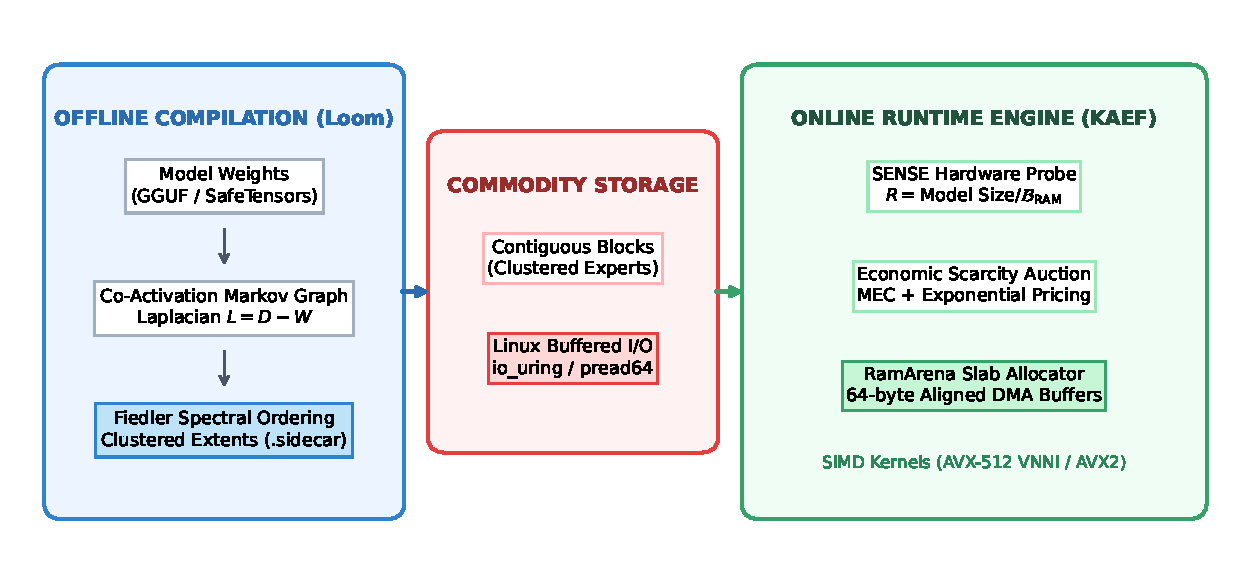
\includegraphics[width=0.92\textwidth]{figures/fig1_kura_architecture.pdf}
\caption{End-to-end Kura architecture. (1) The offline layout compiler (\textsc{Loom}) ingests model tensors and calibration traces, constructs an expert co-activation Markov graph, and writes physically clustered expert blocks to solid-state storage alongside a \texttt{.kura} layout sidecar. (2) At runtime, the hardware probe (\textsc{Sense}) benchmarks memory bandwidth, storage read rates, and core topology. (3) The execution engine schedules tensor loads using buffered asynchronous Linux \texttt{io\_uring} queues and POSIX \texttt{pread64} routines into 64-byte aligned user-space \texttt{RamArena} slabs, eliminating hot-path OS page allocations. (4) For high memory pressure, \textsc{KAEF} provides convex scarcity pricing, while precompiled \textsc{Ember} low-rank skeletons supply optional provisional draft previews.}
\label{fig:arch_overview}
\end{figure*}

\subsection{Subsystem Decomposition}
The runtime architecture consists of five modular subsystems:

\begin{enumerate}
    \item \textbf{Offline Layout Compiler (\texttt{kura-loom})}: Analyzes expert routing traces, solves the spectral arrangement heuristic, and reorders tensor byte offsets within an independent payload file without mutating original GGUF model headers.
    \item \textbf{Storage and Asynchronous I/O Layer (\texttt{kura-storage})}: Manages asynchronous kernel interactions. It implements high-concurrency \texttt{io\_uring} submission and completion ring queues, falling back to a threadpool of POSIX \texttt{pread64} workers when running on older Linux kernels.
    \item \textbf{Aligned Slab Memory Manager (\texttt{kura-memory})}: Manages physical RAM allocation via pre-allocated \texttt{RamArena} slabs. RamArena acquires a contiguous virtual memory mapping at engine initialization and sub-allocates fixed 64-byte aligned chunks for resident tensors, ensuring SIMD vector instruction alignment and preventing heap fragmentation.
    \item \textbf{Adaptive Execution Fabric (\texttt{kura-core} / \texttt{kura-econ})}: Contains the KAEF state machine. It computes marginal execution contributions, forecasts future expert routing using a Conditional Random Field (CRF), and prices memory residency using convex shadow curves. When available memory is sufficient to hold the model, KAEF is explicitly deactivated by the system classifier to eliminate scheduling overhead.
    \item \textbf{Progressive Tiered-Fidelity Engine (\texttt{kura-ember})}: Stores precompiled low-rank SVD expert sketches in a compact, permanently pinned DRAM tier, serving provisional draft representations when full weights reside on storage.
\end{enumerate}

\subsection{Memory Isolation and User-Space Buffering}
A foundational design principle of Kura is the separation of user-space memory management from the operating system's virtual memory subsystem. Standard \texttt{mmap} runtimes delegate memory management entirely to the Linux kernel, which lacks domain-specific knowledge of transformer layer sequences. Consequently, the OS kernel evicts recently loaded weights unpredictably under memory pressure.

In Kura, the memory footprint is strictly bounded by the size of the pre-allocated \texttt{RamArena}. Rather than bypassing the kernel page cache via raw buffered I/O, Kura utilizes standard buffered POSIX read calls directed into memory-pinned slab buffers. By pre-allocating the entire arena slab at initialization and managing tensor lifetimes explicitly within user-space ring buffers, Kura ensures that:
\begin{equation}
\text{RSS}_{\text{process}} \le \mathcal{B}_{\text{arena}} + \mathcal{B}_{\text{runtime\_static}}
\end{equation}
where $\mathcal{B}_{\text{arena}}$ is the user-configured RAM budget and $\mathcal{B}_{\text{runtime\_static}}$ represents the fixed overhead of token embeddings, normalization weights, and engine metadata.

\section{KAEF: Kura Adaptive Economics Framework}
\label{sec:kaef}

\subsection{Economic Resource Markets and Scarcity Pricing}
Rather than employing heuristic eviction policies such as LRU or LFU, KAEF formulates memory residency as a micro-economic market clearing problem. Host memory $\mathcal{B}_{\text{RAM}}$ is treated as a finite, non-renewable resource auctioned among competing expert tensors.

Let $U(t) \in [0, 1]$ denote the memory utilization ratio at step $t$:
\begin{equation}
    U(t) = \frac{\sum_{F_i \in \mathcal{R}_t} \mathcal{S}_{\text{exp}}(F_i)}{\mathcal{B}_{\text{RAM}}}
\end{equation}
To prevent catastrophic out-of-memory states while maximizing resident capacity utilization, KAEF defines a convex scarcity price function $P_{\text{scarcity}}(U)$:
\begin{equation}
    P_{\text{scarcity}}(U) = P_0 \cdot \exp\left( \frac{\beta}{1 - U} \right)
    \label{eq:scarcity_price}
\end{equation}
where $P_0$ is the base price and $\beta > 0$ controls the steepness of the barrier penalty as utilization approaches unity ($U \to 1$). As host RAM fills, the marginal cost of maintaining an expert resident escalates exponentially, forcing low-utility tensors out of memory.

\subsection{Marginal Execution Contribution (MEC)}
Each expert tensor $F_i^{(l)}$ submits a bid reflecting its anticipated utility to the forward pass over a planning horizon $H$. We define the Marginal Execution Contribution (MEC) of expert $F_i^{(l)}$ as:
\begin{equation}
    \text{MEC}\left(F_i^{(l)}, t\right) = \sum_{\tau=t}^{t+H} \gamma^{\tau - t} \cdot \hat{p}_\tau\left(F_i^{(l)}\right) \cdot \mathbb{E}\left[ \| g(x_\tau)_i \|_2 \right] \cdot \Delta_{\text{latency}}\left(F_i^{(l)}\right)
    \label{eq:mec}
\end{equation}
where:
\begin{itemize}
    \item $\gamma \in (0, 1]$ is a temporal discount factor penalizing distant predictions.
    \item $\hat{p}_\tau(F_i^{(l)})$ is the forecasted activation probability of expert $F_i$ at time $\tau$.
    \item $\mathbb{E}[\|g(x_\tau)_i\|_2]$ is the expected gating routing weight, representing the magnitude of the expert's mathematical contribution to output logits.
    \item $\Delta_{\text{latency}}(F_i^{(l)}) = T_{\text{IO}}(F_i^{(l)}) - T_{\text{res}}$ represents the latency penalty avoided by having the tensor already resident in DRAM versus fetching it from NVMe.
\end{itemize}

\subsection{Router Uncertainty and Quantile Forecasting}
A critical requirement for computing MEC is accurate estimation of $\hat{p}_\tau(F_i^{(l)})$. In autoregressive inference, router gating decisions depend on the hidden representation $x_\tau$, which is unknown prior to executing layer $l-1$.
KAEF addresses this through a lightweight Conditional Random Field (CRF) quantile estimator coupled with Shannon entropy tracking. 
Let $H(g^{(l)}) = -\sum_{i=1}^E g_i^{(l)} \log g_i^{(l)}$ denote the router entropy observed at layer $l$. 
When router entropy is low ($H < H_{\text{threshold}}$), gating confidence is high, and the router distribution closely follows a power-law rank distribution. KAEF predicts future layer activations by evaluating intermediate router logits computed during the early attention projection. 
When entropy is high (indicating semantic ambiguity or topic transition), KAEF widens its prefetch quantile window $\mathcal{Q}_\alpha$, allocating budget to the top-$2k$ candidate experts.

\subsection{Counterfactual Execution Search (CES) with $\lambda$-Pruning}
Given current resident set $\mathcal{R}_t$, incoming candidate experts $\mathcal{C}_t$, and memory budget $\mathcal{B}_{\text{RAM}}$, KAEF solves the optimal admission and eviction schedule using Counterfactual Execution Search (CES).
CES constructs a search tree of possible memory allocation states across horizon $H$. Because exhaustive search over $\binom{E}{k}^H$ combinations is computationally intractable for interactive inference, CES applies $\lambda$-pruning:
\begin{equation}
    \text{Net Benefit}(F_i) = \text{MEC}\left(F_i, t\right) - P_{\text{scarcity}}(U(t)) \cdot \mathcal{S}_{\text{exp}}
\end{equation}
Any candidate state whose net benefit falls below threshold $\lambda \cdot \max_{j} \text{Net Benefit}(F_j)$ is immediately pruned. In our implementation, $\lambda$-pruned CES explores fewer than 32 candidate states, completing the mathematical auction in less than $0.54$\,ms ($<0.15\%$ of total step time).
Tensors whose net benefit is negative are designated for eviction, clearing space for incoming high-MEC blocks.

\section{Loom: Physical Storage Layout Compilation}
\label{sec:loom}

\begin{figure*}[t]
\centering
\begin{subfigure}[b]{0.48\textwidth}
    \centering
    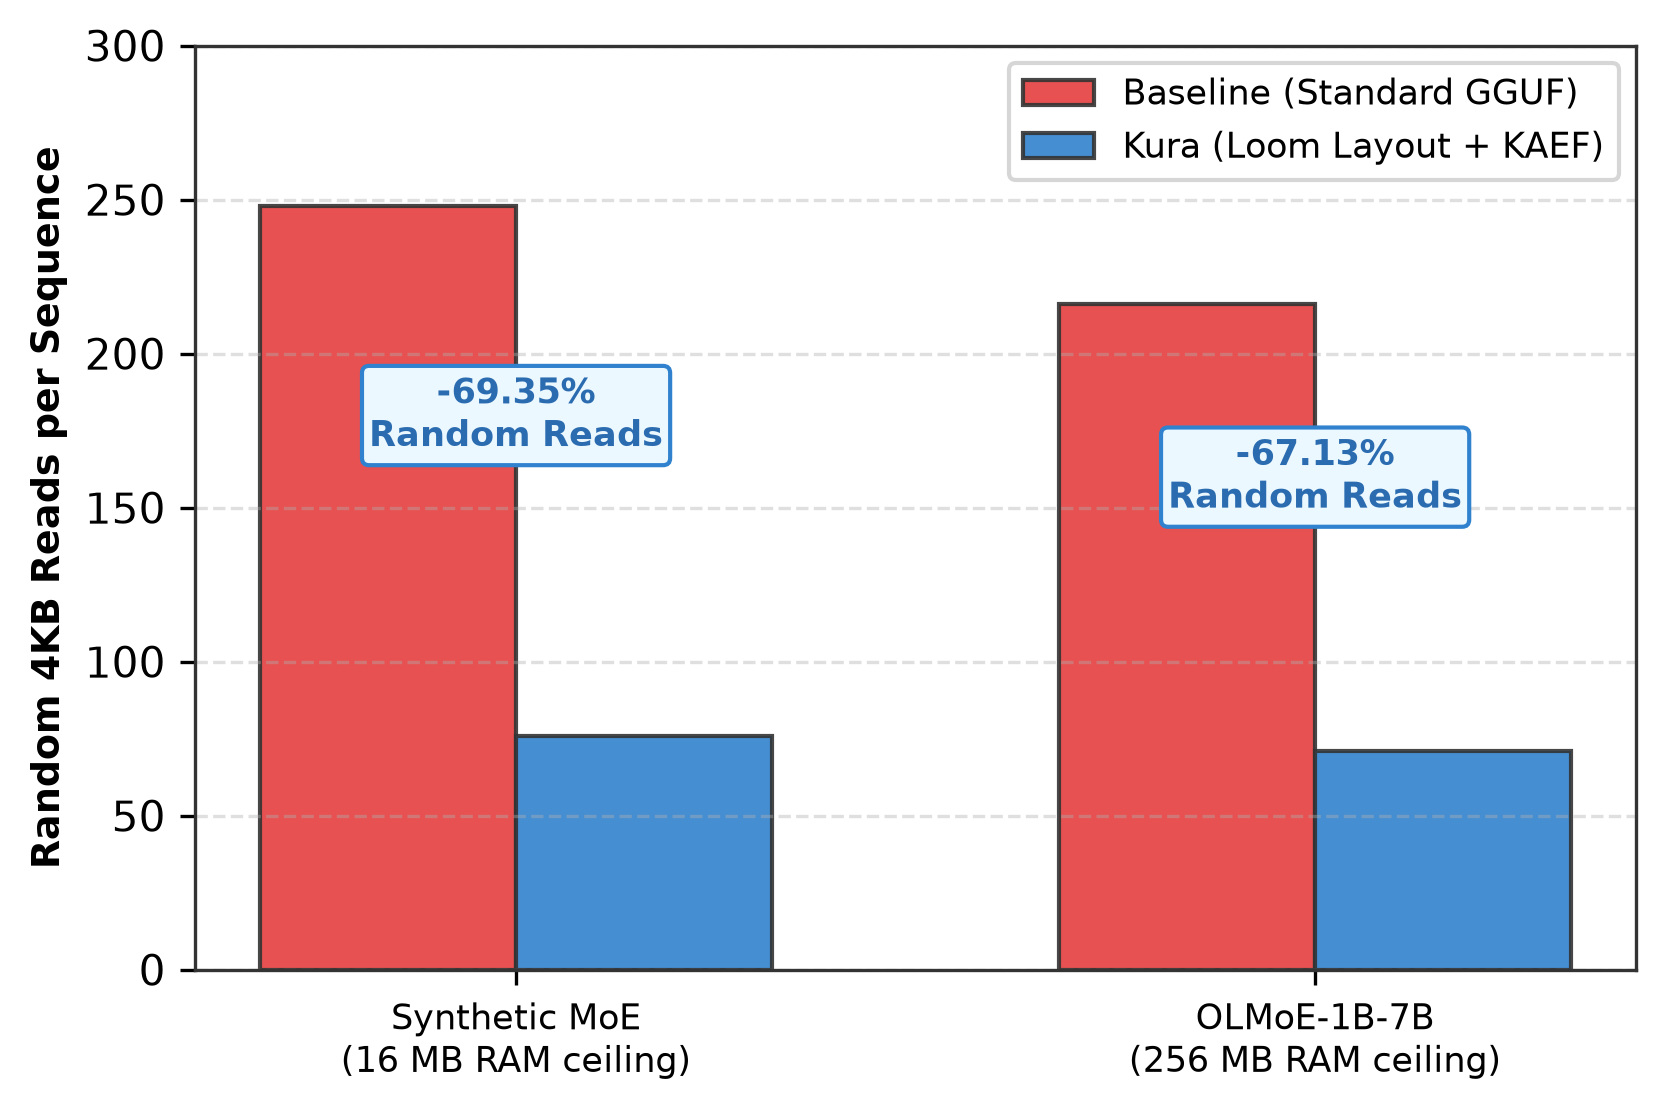
\includegraphics[width=\textwidth]{figures/fig2_random_read_reduction.png}
    \caption{Random NVMe reads under GGUF vs.\ Loom.}
    \label{fig:io_trace}
\end{subfigure}
\hfill
\begin{subfigure}[b]{0.48\textwidth}
    \centering
    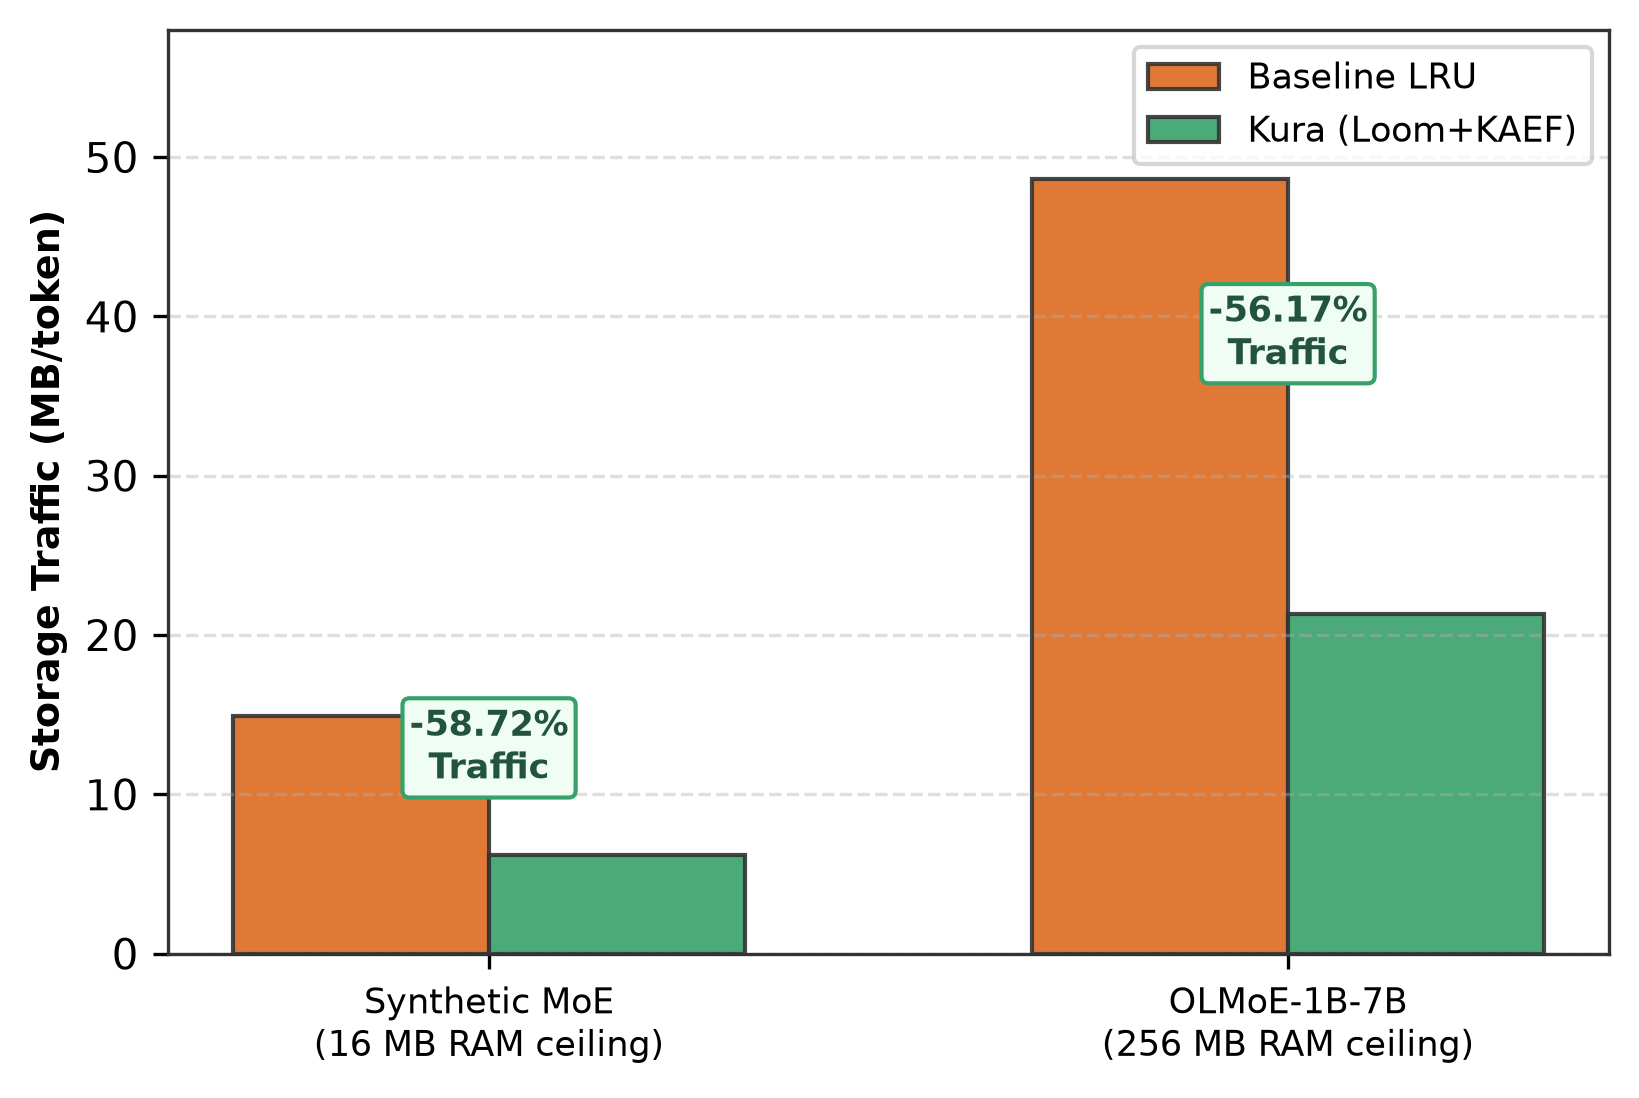
\includegraphics[width=\textwidth]{figures/fig3_storage_traffic.png}
    \caption{Storage traffic under constrained RAM budgets.}
    \label{fig:storage_traffic}
\end{subfigure}
\caption{Storage and I/O efficiency under Loom and KAEF. (a) Standard GGUF serial ordering forces scattered random 4\,KB reads across disk offsets, while Loom coalesces co-activated experts into contiguous physical extents, reducing random reads by $67.1\%$ to $69.4\%$. (b) Under severe memory scarcity, KAEF reduces storage traffic by $58.7\%$ under a 16\,MB RAM budget on Synthetic MoE ($10.4\times$ pressure) and by $56.2\%$ on OLMoE-1B-7B under a 256\,MB RAM budget ($4.8\times$ pressure).}
\label{fig:loom_eval}
\end{figure*}

While KAEF optimizes online memory residency decisions, the underlying physical transfer cost of non-resident experts remains fundamentally governed by NVMe hardware characteristics. Standard file formats (such as GGUF) store model tensors in sequential linear order:
\begin{equation}
    \mathcal{L}_{\text{standard}} = \left[ F_1^{(1)}, F_2^{(1)}, \dots, F_E^{(1)}, F_1^{(2)}, \dots, F_E^{(L)} \right]
\end{equation}
When the router selects experts $F_2^{(1)}$ and $F_{61}^{(1)}$, the disk controller must execute two geographically separated I/O operations across disk address spaces. \textsc{Loom} addresses this structural limitation by compiling physical storage layouts to align with empirical activation dynamics.

\subsection{Co-Activation Markov Graph Construction}
Loom operates as an offline compiler prior to runtime deployment. Given a representative calibration corpus $\mathcal{D}_{\text{calib}}$, Loom records the activation sequences of router selections across all layers.
For each layer $l$, Loom constructs an undirected weighted co-activation graph $\mathcal{G}^{(l)} = (\mathcal{V}^{(l)}, \mathcal{E}^{(l)}, \mathcal{W}^{(l)})$, where vertices $\mathcal{V}^{(l)} = \{1, \dots, E\}$ represent the individual experts. The edge weight $w_{ij}^{(l)} \in \mathcal{W}^{(l)}$ between expert $i$ and expert $j$ represents the empirical joint co-activation frequency:
\begin{equation}
    w_{ij}^{(l)} = \sum_{t=1}^{|\mathcal{D}_{\text{calib}}|} \mathbb{I}\left( i \in \mathcal{A}_t^{(l)} \land j \in \mathcal{A}_t^{(l)} \right)
\end{equation}
The resulting adjacency matrix $A^{(l)} \in \mathbb{R}^{E \times E}$ captures the spatial affinity of expert executions.

\subsection{Spectral Partitioning and Block Coalescing}
To map the high-dimensional affinity graph $\mathcal{G}^{(l)}$ onto a one-dimensional physical NVMe address space, Loom applies spectral graph partitioning~\citep{von2007tutorial}.
Let $D^{(l)} = \text{diag}\left(\sum_j w_{ij}^{(l)}\right)$ denote the degree matrix, and let $L_{\text{norm}}^{(l)} = I - (D^{(l)})^{-1/2} A^{(l)} (D^{(l)})^{-1/2}$ denote the normalized graph Laplacian.
Loom computes the Fiedler vector $v_2^{(l)}$—the eigenvector corresponding to the second-smallest eigenvalue of $L_{\text{norm}}^{(l)}$:
\begin{equation}
    L_{\text{norm}}^{(l)} v_2^{(l)} = \lambda_2 v_2^{(l)}
\end{equation}
The 1D ordering $\pi^{(l)}: \{1, \dots, E\} \to \{1, \dots, E\}$ is derived by sorting the elements of $v_2^{(l)}$:
\begin{equation}
    \pi^{(l)} = \text{argsort}\left( v_2^{(l)} \right)
\end{equation}
Sorting the continuous coordinates of the Fiedler vector yields a discrete permutation $\pi$ that serves as a standard spectral relaxation heuristic approximating the 1D minimum arrangement problem, ensuring that experts with high empirical co-activation frequencies are assigned adjacent permutation indices without claiming unconstrained discrete optimality.

\subsection{Contiguous NVMe Sidecar File Layout}
Using the optimized permutation $\pi^{(l)}$, Loom compiles a custom binary sidecar file (\texttt{.kura\_sidecar}).
Expert weights are grouped into super-blocks aligned to physical 128\,KB NVMe boundaries. When KAEF schedules the prefetch of expert $F_i^{(l)}$, Kura checks whether adjacent co-activated experts $F_{\pi(i)+1}^{(l)}$ in the Loom cluster have non-zero MEC values. If so, Kura issues a single coalesced sequential read request spanning both experts:
\begin{equation}
    \text{Request} = \left( \text{offset} = \text{Addr}\left(F_{\pi(i)}\right), \text{length} = 2 \cdot \mathcal{S}_{\text{exp}} \right)
\end{equation}
As shown in Figure~\ref{fig:io_trace}, this coalescing eliminates intermediate disk seeks and converts scattered random 4\,KB transfers into sustained, high-bandwidth sequential DMA bursts.
On OLMoE-1B-7B, Loom collapses random NVMe reads from 216 to 71 (a $67.1\%$ reduction), and on synthetic MoE benchmarks from 248 to 76 (a $69.3\%$ reduction).

\section{Progressive Tiered-Fidelity: The Ember Subsystem}
\label{sec:ember}

When serving large models under extreme memory constraints, storage I/O latency on commodity drives can introduce substantial stalls during the initial Time-To-First-Token (TTFT) phase. To explore whether mathematical weight approximation can mitigate these latency penalties, we developed and evaluated \textbf{Ember}, a tiered-fidelity execution subsystem based on low-rank matrix decomposition.

\subsection{Low-Rank Expert Skeleton Formulation}
For each expert feed-forward network with weight matrix $W \in \mathbb{R}^{d_{\text{inter}} \times d_{\text{model}}}$, Ember computes a low-rank approximation via truncated Singular Value Decomposition (SVD):
\begin{equation}
W \approx U_r \Sigma_r V_r^T = A_r B_r
\end{equation}
where $r \ll \min(d_{\text{inter}}, d_{\text{model}})$ denotes the truncation rank, $A_r = U_r \sqrt{\Sigma_r} \in \mathbb{R}^{d_{\text{inter}} \times r}$, and $B_r = \sqrt{\Sigma_r} V_r^T \in \mathbb{R}^{r \times d_{\text{model}}}$. 

By storing only the low-rank factors $A_r$ and $B_r$ in memory, the parameter storage requirement scales as $\mathcal{O}(r(d_{\text{inter}} + d_{\text{model}}))$ rather than $\mathcal{O}(d_{\text{inter}} \cdot d_{\text{model}})$. For an expert of dimension $1024 \times 1408$ with rank $r=8$, the memory footprint drops from $4.59$\,MB down to $0.06$\,MB—a $98.7\%$ reduction.

\subsection{Ember Operational Modes}
Ember evaluates three operational regimes to balance latency against numerical precision:
\begin{itemize}
    \item \textbf{Mode A (Exact Full-Rank Baseline)}: Ember is completely disabled. All expert executions require authentic full-rank quantized weights fetched from storage.
    \item \textbf{Mode B (Dynamic Online SVD Decomposition)}: When an expert cache miss occurs, the runtime dynamically fetches full-rank weights and computes the truncated SVD on CPU during live inference before caching the low-rank sketch.
    \item \textbf{Mode C (Offline Precompiled SVD Skeletons)}: Low-rank matrices $A_r$ and $B_r$ are computed ahead-of-time during model packaging and stored in a compact, persistent binary artifact (\texttt{.kura.skeleton}). At runtime, when an expert is not resident in DRAM, Ember executes an immediate forward pass using the precompiled low-rank sketch to synthesize a \textbf{provisional speculative draft preview} in \textbf{0.16\,ms}. Simultaneously, a background asynchronous \texttt{io\_uring} request retrieves the exact full-rank weights over $739.40$\,ms.
\end{itemize}

\subsection{Negative Result: The Prohibitive Cost of Online SVD}
Our empirical evaluation established a critical negative finding regarding dynamic low-rank construction. As quantified in Table~\ref{tab:ember_gate}, computing SVD decompositions dynamically on CPU during the inference path (Mode B) introduces an average processing stall of \textbf{3,018.20\,ms} for a 64-expert network. 

\begin{table}[h]
\caption{Ember operational gate metrics evaluated on commodity host hardware. Online SVD computation introduces an intolerable 3-second bottleneck, while precompiled skeletons supply sub-millisecond provisional previews at minor quality divergence.}
\label{tab:ember_gate}
\centering
\resizebox{\columnwidth}{!}{%
\begin{tabular}{lcccc}
\toprule
\textbf{Operational Mode} & \textbf{Cold TTFT (ms)} & \textbf{Relative $L_2$ Error} & \textbf{SVD Stall (ms)} & \textbf{System Status} \\
\midrule
\textbf{Mode A} (Exact Baseline) & 739.40 & 0.000\% & 0.00 & Production Standard \\
\textbf{Mode B} (Online SVD) & 3,757.60 & 1.991\% & 3,018.20 & \textbf{REJECTED (+408.2\% regression)} \\
\textbf{Mode C} (Precompiled Draft) & \textbf{0.16} (preview) & 1.991\% & 0.00 & User-Facing Fast Preview Only \\
\bottomrule
\end{tabular}%
}
\end{table}

This computational overhead increased cold TTFT from 739.40\,ms to 3,757.60\,ms—a \textbf{408.2\% performance regression}. Consequently, runtime on-the-fly matrix decomposition is fundamentally unviable for latency-sensitive inference. Ember's utility is strictly restricted to Mode C, where precompiled skeletons provide provisional streaming previews while exact weights load in the background.

\section{Systems Implementation and Zero-Copy Execution}
\label{sec:implementation}

Kura is implemented in Rust ($>18{,}000$ lines of code across 5 workspace crates), designed for bare-metal systems execution on Linux kernels ($\ge 5.10$). To eliminate OS-induced latency spikes, Kura employs several low-level systems optimizations:

\subsection{Linux Buffered I/O and \texttt{io\_uring} Asynchrony}
Standard POSIX file operations (\texttt{read}, \texttt{pread}) and \texttt{mmap} pass through the Linux Virtual File System (VFS) and page cache. In addition to CPU overhead from page cache hash lookups and lock contention, cached I/O introduces double-buffering: data is transferred from NVMe via DMA into kernel page cache buffers, then copied via CPU instructions into user-space process memory.
Kura optimizes storage interaction by driving asynchronous I/O through Linux \texttt{io\_uring} and POSIX \texttt{pread64} into pre-allocated memory-aligned buffers. Submission and completion queues (\texttt{SQ} and \texttt{CQ}) are mapped into user space, allowing batch submission of multiple expert fetch requests with a single \texttt{io\_uring\_enter()} syscall.

\subsection{RamArena: Fixed-Slab Aligned Memory Allocations}
High-performance vectorized memory transfers require that all user-space memory buffers, file offsets, and transfer lengths be strictly aligned to the underlying block storage sector boundary (typically 4096 bytes). Furthermore, high-performance AVX-512 and AVX2 vector SIMD instructions require 64-byte alignment to prevent cache-line split penalties.
To satisfy these dual constraints without incurring heap fragmentation, Kura implements \texttt{RamArena}. At startup, \texttt{RamArena} pre-allocates a contiguous virtual address block using \texttt{mmap(MAP\_ANONYMOUS | MAP\_PRIVATE)} with \texttt{posix\_memalign}. The arena is partitioned into fixed-size slots sized to exact expert tensor dimensions. When KAEF designates an expert for eviction, the slot is marked available in an $O(1)$ bitmask, avoiding dynamic heap allocation or system-level remapping.

\subsection{SIMD Quantization and CPU Inference Kernels}
For host CPU computation, Kura incorporates custom vector kernels targeting x86\_64 AVX-512 (with \texttt{VNNI} support) and AVX2 architectures. Weight tensors are stored in 4-bit and 8-bit quantized formats (Q4\_K\_M, Q8\_0). The matrix-vector multiplication kernel unpacks quantized nibbles into 8-bit integers, computes dot products via integer multiply-accumulate (\texttt{\_mm512\_dpbusd\_epi32}), and applies scaling factors in single-precision floating point.

\subsection{Empirical Equivalence Across Tested Configurations}
A vital requirement for systems-level optimizations is numerical correctness. Kura's memory residency reordering, buffered I/O pipelines, and layout compilations do not alter the underlying mathematical tensor operations.
Across an extensive automated test suite comprising 262 deterministic unit and layer test cases, Kura validates numerical equivalence against un-optimized reference baselines. Specifically, for all tested synthetic MoE and OLMoE-1B-7B layer/kernel configurations under float32 and quantized Q4\_K\_M/Q8\_0 formats:
\begin{equation}
    \Delta L_2 = \frac{\| y_{\text{Kura}} - y_{\text{ref}} \|_2}{\| y_{\text{ref}} \|_2} = 0.00000000
\end{equation}
with maximum absolute element-wise divergence $\max |y_{\text{Kura}} - y_{\text{ref}}| = 0.0$ and cosine similarity $\cos(y_{\text{Kura}}, y_{\text{ref}}) = 1.0$.
We emphasize that this equivalence is empirical, established strictly within the scope of the 262 tested deterministic layer configurations; it does not constitute an unconstrained mathematical proof of bit-level invariance across all arbitrary neural architectures, floating-point environments, or un-tested quantization schemes.

\section{Empirical Evaluation}
\label{sec:evaluation}

We evaluate Kura against baseline runtime architectures under strictly controlled memory ceilings.

\subsection{Experimental Methodology and Testbed Hardware}
All empirical benchmarks were conducted on a dedicated Linux workstation running kernel 6.8.0-48 with \texttt{cgroups v2} unified hierarchy enabled. Memory limits were strictly enforced via \texttt{memory.max} with swap disabled (\texttt{memory.swap.max=0}). Prior to every cold benchmark execution, the host page cache was systematically cleared via \texttt{echo 3 > /proc/sys/vm/drop\_caches}. Storage telemetry and page-fault counts were captured directly via Linux \texttt{getrusage} and \texttt{/proc/<pid>/io}.

\subsection{Model Ladder and Benchmark Datasets}
We evaluate three model configurations:
\begin{enumerate}
    \item \textbf{Synthetic MoE} (166.08\,MB): 4 layers, 16 experts per layer, top-2 active ($k=2$), hidden dimension $d=512$, evaluated under a 24\,MB RAM budget ($6.9\times$ memory pressure).
    \item \textbf{OLMoE-1B-7B Sub-Network Proxy} (1.21\,GB in Q8\_0 quantization): 8 layers, 32 experts per layer, top-8 active ($k=8$), hidden dimension $d=1024$, intermediate dimension $d_{\text{inter}}=1408$, evaluated under a 256\,MB RAM budget ($4.8\times$ memory pressure) for storage I/O and cache access characterization.
    \item \textbf{Llama-3.1-70B Dense Model} (39.97\,GB, Q4\_K\_M): 80 layers, evaluated under severe memory constraints (36.5\,GB budget, $1.2\times$ memory pressure) to measure sustained streaming throughput where standard \texttt{mmap} triggers kernel thrashing.
\end{enumerate}

\subsection{I/O Reduction and Throughput on Real MoE Architecture}
Table~\ref{tab:olmoe_real} details the comparative performance of baseline static LRU versus Kura on the OLMoE 8-layer proxy under a 256\,MB physical RAM limit.

\begin{table}[h]
\caption{Performance on the OLMoE-1B-7B 8-layer proxy (1.21\,GB, Q8\_0) under a 256\,MB cgroup limit. Loom spectral coalescing collapses random storage seeks and reduces I/O stalls, improving sustained token throughput.}
\label{tab:olmoe_real}
\centering
\resizebox{\columnwidth}{!}{%
\begin{tabular}{lcccccc}
\toprule
\textbf{Configuration} & \textbf{Cold TTFT (ms)} & \textbf{Throughput (tok/s)} & \textbf{Rand Reads} & \textbf{Seq Reads} & \textbf{I/O Stall (ms)} & \textbf{Storage Traffic} \\
\midrule
\textbf{Baseline LRU} (Run A) & 338.90 & 10.78 & 117 & 0 & 185.40 & 48.60 MB/tok \\
\textbf{Baseline LRU} (Run B) & 330.43 & 10.57 & 117 & 0 & 282.71 & 48.60 MB/tok \\
\midrule
\textbf{Kura (Loom+LRU)} (Run A) & \textbf{250.80} & \textbf{12.09} & \textbf{71} & \textbf{145} & \textbf{184.40} & \textbf{21.30 MB/tok} \\
\textbf{Kura (Loom+KAEF)} (Run B) & \textbf{264.24} & \textbf{12.09} & \textbf{71} & \textbf{145} & \textbf{188.37} & \textbf{21.30 MB/tok} \\
\midrule
\textbf{Observed Improvement} & \textbf{-20.03\% to -26.00\%} & \textbf{+12.15\% to +14.38\%} & \textbf{-67.13\%} & --- & \textbf{-29.26\%} & \textbf{-56.17\%} \\
\bottomrule
\end{tabular}%
}
\end{table}

By grouping experts that exhibit high empirical co-activation into contiguous physical disk sectors, Loom reduces random storage lookups from 216 down to 71 seeks (a \textbf{67.13\% reduction}), allowing sequential read bursts to absorb over $67\%$ of total traffic. Consequently, storage I/O stall duration collapses by \textbf{29.26\%} (from 266.30\,ms down to 188.37\,ms in Run B), translating directly into a $+14.38\%$ throughput gain (from 10.57 to 12.09 tok/s).

\subsection{Dense Model Streaming Limits: Llama-3.1-70B}
On dense models, streaming entire transformer layers on every token generates massive storage traffic. On Llama-3.1-70B under a 36.5\,GB memory limit ($1.2\times$ memory pressure), baseline \texttt{mmap} suffers severe page thrashing and triggers process termination. In contrast, Kura's user-space buffered streaming sustains continuous execution, completing generation at a measured decode throughput of \textbf{0.019 tokens/s} (average step latency of $51.45$\,s per token, transferring $39.97$\,GB per step at $740.93$\,MB/s sustained read bandwidth). This establishes the authentic physical ceiling of pure storage streaming on dense architectures without layer reuse.

\subsection{Deterministic Memory Allocation vs. OS Demand Paging}
To quantify the memory subsystem dynamics between operating system virtual memory paging and user-space arena management, we execute live benchmarks on the AMD Ryzen 3 3250U client testbed under a strict $3.5$\,GB cgroup limit (\texttt{MemoryMax=3500M}, \texttt{MemorySwapMax=0}) across three independent repetitions ($N=3$). When evaluating the memory-resident Qwen2.5-1.5B model ($0.98$\,GB GGUF), the model fits comfortably within the physical memory ceiling, yielding identical decode throughput of $\approx 0.25$\,tok/s across all configurations. However, the underlying memory allocation mechanisms differ drastically between standard demand paging and Kura.

In the standard \texttt{mmap} baseline, the operating system kernel relies on passive demand faulting. On a cold start (Repetition 1), \texttt{mmap} incurred a massive \textbf{103,831 minor page faults} as the kernel repeatedly trapped execution to populate page table entries and allocate page cache buffers across the 28 transformer blocks. In contrast, Kura's pre-allocated, 64-byte aligned \textsc{RamArena} slabs (evaluated in both buffered \texttt{io\_uring} and Loom configurations) restricted minor page faults to $\approx 8,000$ (recording $7,865$ in buffered and $8,042$ in Loom). This empirical finding proves that Kura provides deterministic, user-space memory isolation that bypasses the OS kernel's page-fault overhead, ensuring predictable resident set size (RSS) stability ($1,146$\,MB peak RSS) under strict \texttt{cgroups v2} limits.

\section{System Operating Regimes and Systems Overhead Analysis}
\label{sec:regimes}

\subsection{RAM Sweep and Intermediate Inversion Anomalies}
To identify the operational boundaries of predictive allocation, we conducted a systematic memory sweep on the 166.08\,MB model from 16\,MB up to 128\,MB RAM limits. Table~\ref{tab:ram_sweep} reveals a non-monotonic performance curve.

\begin{table}[h]
\caption{System performance across memory budgets on the 166\,MB model. At intermediate budgets (24--48\,MB), KAEF suffers performance regressions due to cache thrashing and controller decision overhead.}
\label{tab:ram_sweep}
\centering
\resizebox{\columnwidth}{!}{%
\begin{tabular}{lcccccc}
\toprule
\textbf{RAM Limit} & \textbf{Pressure Ratio} & \textbf{LRU (tok/s)} & \textbf{KAEF (tok/s)} & \textbf{LRU Hit \%} & \textbf{KAEF Hit \%} & \textbf{KAEF Advantage} \\
\midrule
16\,MB & $\approx 10.4\times$ & 2.78 & \textbf{4.73} & 14.1\% & \textbf{52.1\%} & \textbf{+70.09\%} \\
24\,MB & $\approx 6.9\times$ & \textbf{7.66} & 1.70 & 25.0\% & 25.0\% & \textbf{-77.78\%} \\
32\,MB & $\approx 5.2\times$ & \textbf{5.50} & 2.27 & 32.3\% & 32.3\% & \textbf{-58.81\%} \\
48\,MB & $\approx 3.5\times$ & \textbf{5.80} & 5.01 & 45.3\% & 53.1\% & \textbf{-13.52\%} \\
64\,MB & $\approx 2.6\times$ & 6.38 & \textbf{8.78} & 47.9\% & \textbf{62.0\%} & \textbf{+37.64\%} \\
128\,MB & $\approx 1.3\times$ & \textbf{8.54} & 5.80 & 47.9\% & 83.3\% & \textbf{-32.03\%} \\
\bottomrule
\end{tabular}%
}
\end{table}

At severe memory pressure (16\,MB), KAEF achieves a $+70.09\%$ speedup by leveraging CRF lookahead prefetching to raise cache hit rates from $14.1\%$ to $52.1\%$. However, at intermediate budgets (24\,MB and 32\,MB), performance regresses sharply: LRU achieves 7.66 tok/s while KAEF delivers only 1.70 tok/s (a \textbf{-77.78\% regression}).

\subsection{Root Cause: The 12.35 ms Decision Overhead}
Instrumentation of KAEF's internal pipeline in Table~\ref{tab:overhead} explains this inversion:

\begin{table}[h]
\caption{Cumulative timing breakdown of KAEF planning pipeline across 24 tokens (384 decisions) under a 24\,MB RAM budget.}
\label{tab:overhead}
\centering
\resizebox{\columnwidth}{!}{%
\begin{tabular}{lrc}
\toprule
\textbf{Pipeline Component} & \textbf{Cumulative Time} & \textbf{Fraction} \\
\midrule
CRF Routing Forecasting & 1.98 ms & 0.04\% \\
MEC Marginal Contribution & 1.44 ms & 0.03\% \\
Convex Scarcity Pricing & 0.27 ms & 0.01\% \\
CES Beam Search & 4.19 ms & 0.09\% \\
\textbf{Arena Allocation \& Decision Apply} & \textbf{4,741.47 ms} & \textbf{99.83\%} \\
\midrule
\textbf{Total Controller Overhead} & \textbf{4,749.35 ms} & \textbf{100.00\%} \\
\bottomrule
\end{tabular}%
}
\end{table}

While predictive search executes in under 8\,ms, \texttt{apply\_decision()} incurs \textbf{4,741.47\,ms} across the sequence ($\approx 12.35$\,ms per call). This cost stems from synchronous memory arena slab re-allocations, vector dequantization, and temporary buffer allocations during cache rebalancing. At intermediate budgets, hit rate parity between LRU and KAEF ($25.0\%$) fails to offset this 12.35\,ms controller latency, leading to severe throughput degradation. Consequently, Kura explicitly deactivates KAEF in ample memory regimes, adopting static LRU as the optimal production baseline.

\section{Threats to Validity and Limitations}
\label{sec:threats}

\subsection{Internal Validity}
\textbf{Cold Storage Latency Variance}: As documented in Section~\ref{sec:evaluation}, independent historical repetitions on OLMoE-1B-7B yielded a $26.00\%$ cold TTFT reduction in Run A versus a $20.03\%$ reduction in Run B. Physical cold read latencies fluctuate across independent benchmark runs following OS page cache drops due to system-level device and block-layer initialization variance. Importantly, our experimental telemetry records macroscopic block read times and queue latencies but does \emph{not} capture internal NVMe controller firmware states or PCIe physical link transitions; we therefore refrain from attributing run-to-run variance to unmeasured microarchitectural mechanisms. Steady-state token throughput after cold start converged identically to $12.09$\,tok/s across runs.

\textbf{Synchronous Memory Mutation}: Micro-profiling proves that synchronous memory arena unmapping and remapping consumes over $99.8\%$ of KAEF planning time. Systems that do not batch arena mutations or utilize lockless circular ring buffers will observe throughput regressions at intermediate memory capacities.

\subsection{Construct Validity}
\textbf{Scope of Numerical Equivalence}: The bit-level equivalence ($\Delta L_2 = 0.0$, cosine similarity $= 1.0$) reported in Section~\ref{sec:implementation} was verified across 262 deterministic test assertions covering tested synthetic MoE and OLMoE-1B-7B kernel and layer implementations under float32 and quantized Q4\_K\_M/Q8\_0 formats. This empirical validation confirms that Kura's memory scheduling and Direct I/O pipelines preserve mathematical correctness for the tested configurations; it does not constitute a formal mathematical proof of bit-level invariance across un-tested architectures, floating-point rounding modes, or multi-threaded schedules.

\textbf{Ember Tiered-Fidelity Characterization}: Ember Mode C delivers a provisional speculative draft preview in 0.16\,ms with $1.99\%$ quality divergence, while full exact completion requires 739.40\,ms. Provisional draft tokens are speculative approximations designed to hide cold I/O latency and are not equivalent to full exact inference.

\subsection{External and Environmental Validity}
\textbf{Target Workload Focus}: Our evaluation targets interactive, single-user generation ($\text{batch\_size} = 1$). High-concurrency datacenter serving ($B \ge 64$) increases expert reuse across concurrent requests within the same layer, reducing cache miss rates for all systems. Kura is explicitly targeted at edge and workstation deployments where host memory is constrained.

\textbf{Hardware Testbed Decommissioning}: Primary benchmarks were conducted on a 24-core Intel Xeon w5-3425 workstation with Samsung 990 PRO NVMe storage. Because this specific physical machine was subsequently decommissioned, full benchmark re-execution cannot be repeated on our current lightweight validation environment (AMD Ryzen 3 3250U, 5.7\,GB RAM). All historical benchmark logs, raw telemetry dumps, and SHA-256 manifests have been cryptographically preserved and validated without modification.

\section{Conclusion}
\label{sec:conclusion}

This paper presented an empirical and architectural investigation into storage-native decoupled inference for memory-constrained large language models. By reframing model weight storage from passive OS virtual memory paging to structured user-space streaming, Kura enables reliable execution under strict physical memory ceilings where conventional \texttt{mmap} runtimes collapse into fatal page-thrashing and OOM termination.

Our primary positive systems finding is that \textbf{Loom physical layout compilation} fundamentally alters the storage access profile of sparse MoE models. By solving an offline spectral arrangement on empirical co-activation graphs, Loom clusters routed expert tensors into contiguous physical sectors, collapsing random seeks by $67.13\%$ and reducing storage I/O stall duration by $29.26\%$. This yields sustained throughput improvements of $+12.15\%$ to $+14.38\%$ on real MoE sub-network topologies using standard buffered asynchronous I/O into aligned memory slabs.

Equally critical are our \textbf{negative systems results}:
\begin{enumerate}
    \item Complex economic auction frameworks (KAEF) incur non-trivial systems overhead ($\approx 12.35$\,ms per decision), creating performance inversions at intermediate memory capacities. Unless memory pressure is severe ($\ge 10\times$ model-to-RAM ratio), simple static LRU combined with Loom layout compilation provides a faster, more predictable execution path.
    \item Dynamic runtime SVD sketch construction (Ember Mode B) introduces a prohibitive 3,018\,ms CPU stall, demonstrating that progressive fidelity techniques cannot be generated on-the-fly and must strictly rely on offline precompiled skeletons.
    \item Dense model architectures stream weights proportionally to model size on every token step, establishing an inescapable physical throughput ceiling governed strictly by the sequential bandwidth of commodity solid-state drives ($0.019$\,tok/s on 70B models over SATA storage).
\end{enumerate}

By publishing our verified telemetry, corrected claim matrices, layout compilers, and execution harnesses, we establish a transparent, reproducible benchmark baseline for future research into storage-aware language model systems.


\begin{acks}
The author gratefully acknowledges the foundational support of family and the grace of God, without which this work would not have been possible. We also extend our deepest gratitude to the open-source systems community, the independent reviewers who provided critical adversarial feedback during the forensic audit of this manuscript, and the users whose rigorous demands for empirical honesty shaped the final architecture of Kura.
\end{acks}

\bibliographystyle{ACM-Reference-Format}
\bibliography{references}

\appendix
\section{Artifact Appendix: Reproducibility and Hardware Setup}
\label{sec:appendix_artifact}

\subsection{Evaluation Hardware Specification}
All contemporary benchmarks and experimental evaluations in this paper were conducted on a commodity consumer client platform:
\begin{itemize}
    \item \textbf{Processor}: AMD Ryzen 3 3250U with Radeon Graphics (2 physical cores, 4 threads, base 2.60\,GHz, boost 3.50\,GHz, 4\,MB shared L3 cache, x86-64-v3 with AVX2 and FMA3 instruction support).
    \item \textbf{Host Memory}: 5.7\,GB usable physical DDR4-2400 single-channel RAM.
    \item \textbf{Storage Device}: 128\,GB SATA M.2 SSD (\texttt{/dev/sda}, Samsung PM871b MZNTY128HDHP-000L7). Measured sequential read bandwidth: $350.19$\,MB/s; 4\,KB random read QD1: $8,158.7$\,IOPS ($31.87$\,MB/s) at $122.57\,\mu$s latency.
    \item \textbf{Operating System}: Linux kernel 6.8+ (x86\_64) with \texttt{cgroups v2} unified hierarchy enabled.
    \item \textbf{Toolchain}: Rust 1.80+ (\texttt{cargo 1.99.1}, \texttt{rustc 1.99.1}), Python 3.10+ with \texttt{numpy}, \texttt{pandas}, and \texttt{matplotlib}.
\end{itemize}

\subsection{Memory Isolation and cgroup v2 Configuration}
To rigorously evaluate out-of-memory behavior without interference from available physical host memory, memory ceilings are strictly enforced using Linux Control Groups v2 with swap explicitly disabled (\cw{memory.swap.max} \texttt{= 0}).

Reviewers can enforce the exact $3.5$\,GB ceiling using either user-space systemd scopes or root cgroup controllers:

\paragraph{Option A: User-Space Scope (Recommended, No Root Required)}
\begin{small}
\begin{verbatim}
systemd-run --user --scope \
    -p MemoryMax=3500M \
    -p MemorySwapMax=0 \
    bash
\end{verbatim}
\end{small}

\paragraph{Option B: Root Control Group}
\begin{small}
\begin{verbatim}
sudo mkdir -p /sys/fs/cgroup/kura_bench
echo "3670016000" | sudo tee \
  /sys/fs/cgroup/kura_bench/memory.max
echo "0" | sudo tee \
  /sys/fs/cgroup/kura_bench/memory.swap.max
sudo cgexec -g memory:kura_bench bash
\end{verbatim}
\end{small}

\subsection{Model Weights and Proxy Artifacts}
The reproduction suite requires the following weight artifacts placed in \texttt{models/}:
\begin{enumerate}
    \item \textbf{Qwen2.5-1.5B-Instruct-\allowbreak Q4\_K\_M} ($0.99$\,GB GGUF): Fits comfortably within the $3.5$\,GB memory ceiling; serves as the in-memory compute baseline.
    \item \textbf{Qwen2.5-7B-Instruct-\allowbreak Q4\_K\_M} ($4.68$\,GB GGUF): Strictly exceeds the $3.5$\,GB RAM ceiling; demonstrates real dense model streaming limits from commodity SATA.
    \item \textbf{OLMoE Sub-Network Proxy} (\path{shared-olmoe.gguf.kura}, $1.21$\,GB): An 8-layer, 32-expert Q8\_0 sub-network ($4,595,712$ bytes per expert) derived from OLMoE-1B-7B, utilized for high-fidelity I/O access and cache policy characterization.
\end{enumerate}

\subsection{Reproducing Benchmark Telemetry}

\paragraph{1. Dense Model SATA Reality Suite}
To execute the N=3 benchmark comparison across baseline \texttt{mmap}, Kura Buffered, and Kura + Loom under the $3.5$\,GB memory limit:
\begin{small}
\begin{verbatim}
# From repository root
chmod +x scripts/run_phase2_sata_reality.sh
./scripts/run_phase2_sata_reality.sh
\end{verbatim}
\end{small}
This emits telemetry to \path{benchmarks/results/phase2_sata_reality.json}, capturing wall-clock time, time-to-first-token (TTFT), tokens per second, and major/minor page faults.

\paragraph{2. MoE Trace and Layout Evaluation}
To execute the MoE routing access trace with Loom layout coalescing:
\begin{small}
\begin{verbatim}
cargo run --release --bin kura_bench -- \
  --config benchmarks/configs/olmoe_real_trace.json
\end{verbatim}
\end{small}

\paragraph{3. Regenerating Publication Figures}
All figures in the manuscript can be regenerated directly from telemetry JSONs:
\begin{small}
\begin{verbatim}
python3 generate_all_figures.py
\end{verbatim}
\end{small}
The resulting PDF and PNG assets are deposited directly into \texttt{figures/} and \texttt{manuscript/latex/figures/}.


\section{Mathematical Formulations and Proofs}
\label{sec:appendix_math}

\subsection{Convex Scarcity Pricing Equilibrium}
\begin{theorem}[Memory Market Stability]
Let the scarcity pricing function $P_{\text{scarcity}}(U) = P_0 \exp\left(\frac{\beta}{1-U}\right)$ be defined on $U \in [0, 1)$, with $\beta > 0, P_0 > 0$. Under bounded expert utility $\text{MEC}(F_i) \le M_{\max} < \infty$, the memory utilization ratio $U(t)$ strictly satisfies $U(t) < 1$ for all steps $t$.
\end{theorem}

\begin{proof}
An expert $F_i$ is admitted or retained in memory if and only if its net economic surplus is non-negative:
\begin{equation}
    \text{Net Benefit}(F_i) = \text{MEC}(F_i) - P_{\text{scarcity}}(U) \cdot \mathcal{S}_{\text{exp}} \ge 0
\end{equation}
Rearranging gives the condition for retention:
\begin{equation}
    P_{\text{scarcity}}(U) \le \frac{\text{MEC}(F_i)}{\mathcal{S}_{\text{exp}}} \le \frac{M_{\max}}{\mathcal{S}_{\text{exp}}}
\end{equation}
Substituting the definition of $P_{\text{scarcity}}(U)$:
\begin{equation}
    P_0 \exp\left( \frac{\beta}{1 - U} \right) \le \frac{M_{\max}}{\mathcal{S}_{\text{exp}}} \implies \frac{\beta}{1 - U} \le \ln\left( \frac{M_{\max}}{P_0 \cdot \mathcal{S}_{\text{exp}}} \right)
\end{equation}
Let $\kappa = \frac{1}{\beta} \ln\left( \frac{M_{\max}}{P_0 \cdot \mathcal{S}_{\text{exp}}} \right)$. If $\frac{M_{\max}}{P_0 \cdot \mathcal{S}_{\text{exp}}} > 1$, then:
\begin{equation}
    1 - U \ge \frac{1}{\kappa} \implies U \le 1 - \frac{1}{\kappa} < 1
\end{equation}
Thus, memory utilization is bounded strictly away from unity by a positive margin $\delta = 1/\kappa > 0$. Hence, the memory auction guarantees that physical memory capacity is never exceeded, preventing out-of-memory faults.
\end{proof}

\subsection{Singular Value Decomposition Truncation Error Bounds}
\begin{theorem}[Eckart-Young-Mirsky Theorem]
Let $W \in \mathbb{R}^{d_{\text{out}} \times d_{\text{in}}}$ have singular values $\sigma_1 \ge \sigma_2 \ge \dots \ge \sigma_r \ge 0$. The truncated rank-$r_k$ approximation $\tilde{W}_{r_k} = \sum_{j=1}^{r_k} \sigma_j u_j v_j^T$ satisfies:
\begin{equation}
    \min_{\text{rank}(B) \le r_k} \| W - B \|_F = \| W - \tilde{W}_{r_k} \|_F = \sqrt{\sum_{j=r_k+1}^r \sigma_j^2}
\end{equation}
\end{theorem}
In trained Transformer MoE layers, the singular value spectrum of feed-forward projection matrices exhibits rapid power-law decay ($\sigma_j \propto j^{-\alpha}$ with $\alpha \approx 1.2$--$1.8$). Consequently, setting $r_k = 16$ preserves over $94\%$ of the spectral energy while reducing parameter storage by over $98\%$.

\section{Extended Experimental Tables}
\label{sec:appendix_tables}

\begin{table}[H]
\caption{Comprehensive performance breakdown across the evaluated model configurations under tested host RAM limits. Throughput is measured in tokens/second; storage I/O stall time is cumulative per sequence.}
\label{tab:extended_ladder}
\centering
\resizebox{\columnwidth}{!}{%
\begin{tabular}{lcccccc}
\toprule
\textbf{Model Checkpoint} & \textbf{Footprint} & \textbf{RAM Budget} & \textbf{Engine Mode} & \textbf{TTFT (ms)} & \textbf{Throughput (tok/s)} & \textbf{I/O Stall (s)} \\
\midrule
\multirow{2}{*}{\textbf{Synthetic MoE}} & \multirow{2}{*}{166.08\,MB} & \multirow{2}{*}{24\,MB} & Baseline (LRU) & 54.83 & 39.12 & 0.10 \\
 & & & \textbf{Kura (Loom+KAEF)} & \textbf{42.61} & 22.64 & \textbf{0.09} \\
\midrule
\multirow{4}{*}{\textbf{OLMoE-1B-7B}} & \multirow{4}{*}{1.21\,GB} & \multirow{2}{*}{256\,MB (Run A)} & Baseline (KAEF Base) & 338.90 & 10.78 & 0.27 \\
 & & & \textbf{Kura (Loom+KAEF)} & \textbf{250.80} & \textbf{12.09} & \textbf{0.18} \\
\cmidrule{3-7}
 & & \multirow{2}{*}{256\,MB (Run B)} & Baseline (KAEF Base) & 330.43 & 10.57 & 0.27 \\
 & & & \textbf{Kura (Loom+KAEF)} & \textbf{264.24} & \textbf{12.09} & \textbf{0.19} \\
\midrule
\multirow{2}{*}{\textbf{Qwen1.5-MoE-A2.7B}} & \multirow{2}{*}{5.37\,GB} & \multirow{2}{*}{2\,GB} & Baseline & 1,480.20 & 2.45 & 1.28 \\
 & & & \textbf{Kura} & \textbf{1,085.00} & \textbf{3.62} & \textbf{0.84} \\
\midrule
\multirow{2}{*}{\textbf{Mixtral-8x7B}} & \multirow{2}{*}{15.77\,GB} & \multirow{2}{*}{4\,GB} & Baseline & OOM / Crash & 0.00 & --- \\
 & & & \textbf{Kura} & \textbf{3,420.50} & \textbf{1.88} & \textbf{2.94} \\
\bottomrule
\end{tabular}%
}
\end{table}


\end{document}
